% #############################################################################
% This is Chapter 1
% !TEX root = ../main.tex
% #############################################################################
% Change the Name of the Chapter i the following line
\fancychapter{Introduction}
\cleardoublepage
\label{chap:intro}


%\section{Background and Motivation}


Despite decades of research and improved satellite capabilities, the attribution of methane variability to specific environmental drivers remains a critical gap. Although bottom-up inventories describe source processes and \gls{top_down} inversions infer fluxes from concentration data, the causal relationships between observed methane dynamics and factors such as land cover, meteorology, and atmospheric chemistry are poorly constrained. This gap limits our ability to diagnose interpretable emission trends, verify mitigation policies, and anticipate future changes under evolving climate conditions.

This section synthesizes the scientific rationale behind the need for a causal approach to methane analysis, highlighting key atmospheric processes, satellite retrieval capabilities, and the limitations of current correlational studies. Building on this foundation, the subsequent sections develop a framework that integrates causal inference methods with satellite time series data to address attribution challenges in a statistically rigorous manner.

\section{Methane in the Earth System}

Methane (\ch{CH_4}), a colorless and odorless gas, plays a critical role in Earth's atmospheric and climatic systems. It is the second most important contributor to post-industrial radiative forcing after carbon dioxide, with a global warming potential (GWP) 28--34 times greater than \ch{CO_2} on a 100-year horizon \cite{tian_catalytic_2021, IPCC2013}. Unlike carbon dioxide, methane has a shorter atmospheric lifetime of about 9--12 years, which makes it a particularly effective target for near-term climate mitigation \cite{Shindell2012, Etminan2016}. 

Methane exerts both direct and indirect \gls{rf}, the latter through the formation of tropospheric ozone and stratospheric water vapor. It is also a major sink for hydroxyl radicals (OH), which are central to the atmospheric oxidation capacity. These properties make \ch{CH_4} not only a potent greenhouse gas but also a key player in atmospheric chemistry \cite{Shindell2012, Etminan2016}. Reducing methane emissions has the added benefit of improving air quality by decreasing background ozone concentrations.

Methane's sources include both natural and anthropogenic emissions, while sinks are dominated by atmospheric oxidation and soil uptake \cite{Saunois2020, global_methane_budget}. Methane exhibits marked spatial and temporal variability driven by seasonality, geography, and episodic perturbations \cite{Pandey2017, feng_tropical_2022}. Its global distribution is observed through ground-based networks, aircraft campaigns, and increasingly through satellite remote sensing \cite{Jacob2022, Lorente2021, Schneising2019}.

\subsection{Methane Sources and Atmospheric Dynamics} 
\label{sec:ch4-sources-dynamics}

Methane (CH$_4$) is emitted to the atmosphere from a variety of natural and anthropogenic sources, and its observed variability reflects a complex interplay of surface emissions, chemical sinks, and transport processes. While Figure~\ref{fig:methane-mindmap-2020} summarizes the bottom-up estimates, Table~\ref{tab:methane_emissions_2020} provides a more complete breakdown of global methane emissions by source category, based on the 2020 update of the Global Methane Budget \cite{global_methane_budget}.

\begin{figure*}[!ht]
\caption[Global methane emissions by source (2020)]{Breakdown of annual global methane emissions in 2020 by contributor, based on bottom-up estimates (Tg CH\textsubscript{4} yr\textsuperscript{-1}). The mindmap illustrates the relative contributions of direct anthropogenic sources. Values represent category means from the Global Methane Budget \cite{global_methane_budget}.}
\label{fig:methane-mindmap-2020}
\centering
\begin{tikzpicture}[mindmap, grow cyclic, every node/.style=concept, concept color=orange!40, 
    level 1/.append style={level distance=5cm,sibling angle=55},
    level 2/.append style={level distance=3.5cm,sibling angle=45},
    level 3/.append style={level distance=2.5cm,sibling angle=30}]

\node{Methane Emissions \\Total: 685 Tg}
  child [concept color=purple!50] { 
    node {Direct Anthropogenic\\(372)}
      child {node {Fossil Fuels (128)}
        child {node {Coal Mining (41)}}
        child {node {Oil \\ \, \& Gas (74)}}
        child {node {Industry (5)}}
        child {node {Transport (2)}}}
      child {node {Agriculture and Waste (211)}
        child {node {Livestock \\ \& Manure (117)}}
        child {node {Rice Cultivation (32)}}
        child {node {Landfills \\ \& Waste (71)}}}
      child {node {Biomass \\ \& Biofuel (27)}
        child {node {Biomass Burning (17)}}
        child {node {Biofuel Burning (10)}}}
  }
  child [concept color=blue!30] {
    node {Natural and Indirect Anthropogenic (314)}
      child {node {Wetlands \\ \& Inland Waters (251)}
        child {node {Wetlands (161)}}
        child {node {Freshwaters (112)}}}
      child {node {Other Natural (63)}}};
\end{tikzpicture}
\end{figure*}

Emissions are presented as both bottom-up estimates, derived from process-based inventories and field measurements, and top-down estimates, inferred from atmospheric inversions constrained by surface and satellite observations. The sources are grouped into direct anthropogenic emissions, dominated by agriculture, waste management, fossil fuel extraction, and biomass combustion, and natural or indirectly anthropogenic emissions, primarily from wetlands, inland waters, and other ecosystems.

Global methane emissions are estimated at 608--685~Tg\,CH$_4$/yr when combining bottom-up process inventories with top-down atmospheric inversions \cite{global_methane_budget}. Total emissions from bottom-up estimates reached 685~\gls{tg_ch4_yr}, with 372~Tg attributed to direct anthropogenic sources and 314~Tg to natural and indirect anthropogenic sources. Anthropogenic emissions are dominated by fossil fuel activities (128~Tg), agriculture and waste management (211~Tg), and biomass and biofuel combustion (27~Tg). Natural contributions are primarily from wetlands and inland freshwater systems (251~Tg), with an additional 63~Tg from geological seepage, termites, wildfires, and permafrost.

\begin{longtable}{@{} p{8cm} p{3cm} p{3cm} @{} }
\caption{Annual global methane emissions by source category (Tg CH\textsubscript{4} yr\textsuperscript{-1}). \textbf{Bottom-up} values come from process-based inventories and biogeochemical models, whereas \textbf{Top-down} values are derived from atmospheric inversions constrained by surface and satellite CH\textsubscript{4} measurements. Table adapted from the Global Methane Budget 2020 framework \cite{global_methane_budget}.}
\label{tab:methane_emissions_2020} \\
\toprule
\textbf{Source Category} & \textbf{Bottom-Up} & \textbf{Top-Down} \\
\midrule
\endfirsthead
\toprule
\textbf{Source Category} & \textbf{Bottom-Up Estimate} & \textbf{Top-Down Estimate} \\
\midrule
\endhead
\midrule
\multicolumn{3}{r}{\small\textit{Table~\ref{tab:methane_emissions_2020} continued on next page}} \\
\midrule
\endfoot
\bottomrule
\endlastfoot
\textbf{$\blacktriangleright$ Natural and indirect anthropogenic sources} & & \\
$\triangleright$ Combined wetlands and inland freshwaters & 251 [171--364] & 175 [151--229] \\
\hspace{2em}$\bullet$ Wetlands & 161 [131--198] & 175 [151--229] \\
\hspace{2em}$\bullet$ Inland freshwater systems\textsuperscript{1} & 112 [49--202] & -- \\
$\triangleright$ Other natural sources & 63 [24--93] & 44 [40--47] \\
\hspace{2em}$\bullet$ Geological, wild animals, termites, wildfires, permafrost & -- & -- \\
$\triangleright$ Coastal and oceanic sources (biogenic, geologic offshore) & -- & -- \\
\textbf{$\blacktriangleright$ Total natural and indirect anthropogenic} & 314 [195--457] & 216 [193--241] \\
\addlinespace[1.2em]
\textbf{$\blacktriangleright$ Direct anthropogenic sources} & & \\
$\triangleright$ Agriculture and waste & 211 [204--216] & 245 [232--259] \\
\hspace{2em}$\bullet$ Agriculture (total) & 147 [143--149] & -- \\
\hspace{3em}-- Livestock and manure & 117 [114--124] & -- \\
\hspace{3em}-- Rice cultivation & 32 [29--37] & -- \\
\hspace{2em}$\bullet$ Landfills and waste & 71 [60--84] & -- \\
$\triangleright$ Fossil fuels (total) & 128 [120--133] & 122 [101--133] \\
\hspace{2em}$\bullet$ Coal mining & 41 [38--43] & -- \\
\hspace{2em}$\bullet$ Oil and gas & 74 [67--80] & -- \\
\hspace{2em}$\bullet$ Industry & 5 [1--8] & -- \\
\hspace{2em}$\bullet$ Transport & 2 [1--3] & -- \\
$\triangleright$ Biomass and biofuel burning & 27 [20--41] & 26 [22--27] \\
\hspace{2em}$\bullet$ Biomass burning & 17 [13--27] & -- \\
\hspace{2em}$\bullet$ Biofuel burning & 10 [7--14] & -- \\
\textbf{$\blacktriangleright$ Total direct anthropogenic} & 372 [345--409] & 392 [368--409] \\
\addlinespace[1.2em]
\textbf{Total methane sources} & 685 [540--865] & 608 [581--627] \\
Total sinks & 633 [507--796] & 575 [566--589] \\
Source--sink imbalance & 52 & 32 [15--38] \\
Atmospheric growth\textsuperscript{2} & -- & 41.8 [40.7--42.9] \\
\end{longtable}

\vspace{-1.5em}
\begin{flushleft}
{\footnotesize
\textbf{Notes:} \\
1. Inland freshwater systems include lakes, ponds, reservoirs, streams, and rivers. Emissions from these systems may be enhanced by anthropogenic activity.\\
2. Atmospheric growth is derived using a conversion factor of 2.75 Tg CH\textsubscript{4} ppb\textsuperscript{-1} (Prather et al., 2012).\\
3. Values are reported as mean with [min--max] uncertainty ranges. Double counting corrections (e.g., wetlands vs. freshwater systems) are applied in totals but not listed separately.\\
4. Coastal/oceanic emissions and minor natural sources (e.g., wild animals, termites, permafrost) are not separately quantified here.\\
5. Top-down values are global inversions constrained by surface and satellite data. Bottom-up values sum process-based inventories.
}
\end{flushleft}

Notably, inland freshwater systems and coastal/oceanic sources, though often overlooked, contribute significantly to overall emissions in bottom-up assessments, while top-down estimates show less variability across these categories. The reported values include uncertainty ranges, and the totals account for overlaps (e.g., between wetlands and freshwater systems) through internal corrections, although these are not listed separately. This dual-perspective tabulation highlights both the progress and the persistent gaps in global CH\textsubscript{4} accounting, reinforcing the need for integrated observation-modeling approaches in future causal attribution studies.

Natural and indirect anthropogenic sources contribute 195--457~Tg/yr in bottom-up estimates, but only 193--241~Tg/yr in top-down inversions, reflecting substantial uncertainty in wetland and inland freshwater fluxes. Wetlands alone emit 131--198~Tg/yr, with interannual variability strongly tied to precipitation and temperature \cite{Pandey2017, Knox2024}. Inland freshwater systems (lakes, rivers, reservoirs) are increasingly recognized as large emitters, with bottom-up estimates of 49--202~Tg/yr, although top-down constraints are lacking.

Direct anthropogenic sources contribute 345--409~Tg/yr (bottom-up) or 368--409~Tg/yr (top-down) \cite{global_methane_budget}. Agriculture and waste dominate, with 204--216~Tg/yr bottom-up but 232--259~Tg/yr top-down. Within this category, livestock and manure contribute about 114--124~Tg/yr, rice cultivation 29--37~Tg/yr, and landfills plus wastewater 60--84~Tg/yr. Fossil fuels add 120--133~Tg/yr (bottom-up) or 101--133~Tg/yr (top-down), split among coal mining ($\sim$38--43~Tg/yr), oil and gas operations (67--80~Tg/yr), and smaller contributions from industry and transport. Biomass and biofuel burning contributes 20--41~Tg/yr, consistent across both bottom-up and top-down methods.

More recent analyses indicate that agricultural and fossil fuel sources have contributed roughly equal shares to the renewed CH$_4$ growth in the past decades \cite{Jackson_2020}. In the following, we review the key source processes and the atmospheric dynamics that modulate methane's distribution, providing context for causal modeling of methane variability in satellite observations.

\subsection{Biogeochemical Source Processes}

Natural wetlands are the single largest methane source category, responsible for roughly one-fifth to one-third of global emissions under present-day climate. Wetland CH$_4$ is produced by methanogenic archaea in waterlogged, oxygen-depleted soils. Key controls on wetland methane production include soil temperature and redox conditions, the availability of organic substrates, and the depth and extent of inundation. Emissions are modulated by both microbial production and oxidation in situ: methane formed in anaerobic peat or sediments can be partly consumed by methanotrophic bacteria in overlying oxic layers.

The net flux to the atmosphere occurs via three pathways: diffusion through soil and water, \gls{ebullition} (bubbling) when methane accumulates in bubbles, and plant-mediated transport through aerenchymatous vegetation. Because these processes respond non-linearly to environmental drivers, wetland emissions exhibit pronounced seasonal and interannual variability. For instance, extensive flooding and anomalously cool temperatures during the strong \gls{la_nina} of 2011 led to a ~5\% increase in global wetland CH$_4$ emissions, consistent with satellite observations and inverse modeling. Such climate-driven pulses underscore the importance of wetlands in year-to-year methane fluctuations and represent a potential positive feedback with future warming.

Agricultural activities are the dominant anthropogenic methane sources, with livestock and rice cultivation being particularly significant \cite{Jackson_2020}. Enteric fermentation in ruminant livestock (cattle, sheep, goats) produces CH$_4$ as microbes decompose cellulose in the animal's rumen; this methane is exhaled or belched by the animal. Globally, enteric emissions (including manure management) are on the order of 110~Tg~CH$_4$/yr, and have grown with increasing livestock populations and farming intensification. Manure storage under anaerobic conditions (e.g. in lagoons) further contributes to this source.

Rice paddies, which account for about 8--10\% of anthropogenic CH$_4$, emit methane during the growing season when fields are flooded. Flooding creates anoxic soil conditions similar to natural wetlands, enabling methanogenesis in rice soils. Management practices strongly influence rice methane fluxes: intermittent drainage (rather than continuous flooding) allows oxidation of soil CH$_4$ and can suppress emissions, whereas organic amendments (e.g. rice straw) and warm temperatures enhance production. Global rice emissions have been estimated around 25--40~Tg~CH$_4$/yr in recent decades, with most coming from South and East Asia. Notably, trends in rice methane output have declined slightly in some regions due to improved water management and declines in paddy area.

Fossil fuel related emissions (from coal mining, natural gas and oil systems) are another major anthropogenic contributor, responsible for roughly 90--130~Tg~CH$_4$ annually. Methane of thermogenic origin is released during the extraction, processing, and transport of fossil fuels. In underground coal mines, CH$_4$ is vented from coal seams; in oil and gas operations, methane can leak from wellbores, processing equipment, and pipelines, or be deliberately vented and flared. ``Super-emitter'' events (e.g. pipeline ruptures or blowouts) can episodically release large quantities of methane, while diffuse, chronic leakage across vast gas infrastructure contributes a continuous background source. Technological and regulatory measures (such as improved well completion, leak detection and repair) have the potential to mitigate these emissions. Indeed, regional studies show significant variability in oil/gas CH$_4$ loss rates, suggesting that a portion of this source is controllable. Bottom-up inventories and satellite data inversions indicate fossil emissions and agricultural emissions have grown comparably in the 21st century, each explaining roughly 50\% of the anthropogenic increase since 2007.

Biomass burning constitutes a smaller source of methane, on the order of $\sim$20--40~Tg~CH$_4$/yr, but can dominate the CH$_4$ budget of certain regions or periods (e.g. during extreme wildfire seasons). Methane is produced by incomplete combustion of organic material; thus, wildfires, agricultural residue burning, and biofuel use all emit CH$_4$ along with CO$_2$ and CO. The fraction of carbon released as CH$_4$ depends on combustion efficiency, flame temperature, and oxygen availability in the fire. Smoldering fires in peatlands or tropical forests, for example, tend to have higher CH$_4$/CO$_2$ ratios than fast-moving grassland fires. Globally, fire emissions of methane vary interannually with climate: intense El~Niño-induced droughts, such as in 2015--2016, can lead to above-average biomass burning in equatorial Asia and elsewhere, temporarily boosting atmospheric CH$_4$. Conversely, a decline in deforestation and peat fires in the early 2000s has been implicated in a slowing of CH$_4$ growth during that period. Because a large fraction of biomass burning is human-initiated (for land clearance or agriculture), it straddles the line between natural and anthropogenic source categories. Emission inventories typically include wildfires and biofuel use together for completeness.

Other natural sources make up a smaller portion of the methane budget. Termites produce CH$_4$ through microbial digestion of wood and plant matter in their guts, emitting on the order of 5--15~Tg~CH$_4$/yr. Although minor globally ($<$3\% of total emissions), termite methane can be significant in tropical ecosystems with abundant termite mounds. Geological CH$_4$ emissions occur from natural gas seeps and mud volcanoes on land and in the ocean, releasing old (often isotopically heavier, thermogenic) methane from subsurface reservoirs. Recent estimates put the global geological source (including submarine seeps) at roughly 30--60~Tg~CH$_4$/yr, though this is an area of active research and debate. Oceanic biogenic methane (produced by microbes in sediments or anoxic pockets of the ocean water column) contributes only a few teragrams per year to the atmosphere, as most marine CH$_4$ is oxidized by bacteria before reaching the sea-air interface.

Finally, soils generally act as a net sink for atmospheric methane rather than a source: well-drained upland soils harbor methanotrophic bacteria that consume an estimated 30--45~Tg~CH$_4$ annually, partially offsetting other emissions. This soil sink is enhanced in aerobic environments and tends to increase with higher atmospheric CH$_4$ concentration (since diffusion into soils is greater) \cite{global_methane_budget}. The balance between all these diverse sources and sinks determines methane's atmospheric burden and trends.

\subsection{Atmospheric Methane Dynamics and Transport}

Once emitted, methane is mixed and transported through the atmosphere, and ultimately removed by chemical processes. The dominant sink of CH$_4$ is oxidation by the hydroxyl radical (OH) in the troposphere. Globally, 85--90\% of methane removal occurs via the reaction CH$_4$ + OH $\rightarrow$ CH$_3$ + H$_2$O, which effectively gives methane an atmospheric lifetime of about 9 years. This oxidation is most rapid in the tropical mid-troposphere, where warm temperatures, high water vapor, and strong sunlight favor OH production. 

The principal removal pathway is the reaction:
\[ \ch{CH_4 + OH -> CH_3 + H_2O}. \]
This initiates a series of reactions that eventually oxidize methane to \ch{CO_2} and water, consuming about 500~Tg\,CH$_4$/yr \cite{chen_estimation_2006}. OH abundance is controlled by temperature, humidity, and the presence of other reactive gases, making methane's sink strength climate-sensitive. Secondary effects include enhanced tropospheric ozone and additional stratospheric water vapor, which amplify greenhouse forcing and influence stratospheric chemistry \cite{Etminan2016, Shindell2012}.

Minor sinks include reaction with chlorine radicals (mainly in the marine boundary layer) and oxidation in the stratosphere by OH, O($^1$D), and Cl, which together account for $\sim$10--15\% of CH$_4$ loss. The soil sink, as noted, removes a further 30~Tg~CH$_4$/yr (about 5\% of total sink) via microbial uptake in well-aerated soils. Methanotrophic bacteria in upland, well-aerated soils consume methane at atmospheric concentrations. This sink accounts for about 30~Tg\,CH$_4$/yr (5--10\% of the global sink) \cite{Saunois2020, global_methane_budget}. Uptake efficiency depends on soil texture, aeration, and land use, with forest and grassland soils generally showing higher uptake rates \cite{Serata2023}. Although smaller than the OH sink, soil uptake is regionally significant and sensitive to ecosystem change.

Overall, the total global sink is estimated at roughly 550--600~Tg~CH$_4$/yr, approximately balancing the source strength in the current steady state. Changes in OH concentrations can therefore significantly affect methane's growth rate. Indeed, some studies suggest that a small decline in OH (~2--5\%) after 2000 played a substantial role in the post-2007 methane increase, while other analyses of isotopic evidence attribute the renewed growth more to rising microbial emissions than to sink variation. This ambiguity remains a subject of active research, as OH itself is influenced by methane (through feedbacks in tropospheric chemistry) creating a coupled source-sink system.

Methane released at the surface is transported vertically and horizontally by atmospheric motions. Convective uplift and boundary-layer mixing can rapidly carry CH$_4$ from the surface into the free troposphere, where it becomes part of the general circulation. In the troposphere, methane is often treated as a well-mixed gas; however, discernible gradients exist vertically and between hemispheres due to the distribution of sources and sinks.

The Northern Hemisphere (NH) has 90--100~ppb higher CH$_4$ concentrations than the Southern Hemisphere (SH) on average, reflecting the preponderance of anthropogenic sources in the NH (where most land and human activity is located). Airflow between hemispheres is relatively slow (interhemispheric exchange takes 1--2 years), so methane emitted in the NH gradually diffuses to the SH, being partially removed by OH along the way. This yields a persistent interhemispheric gradient with higher CH$_4$ in the NH extratropics and a slump toward the remote southern latitudes.

Transport model analyses using satellite data have identified key pathways for interhemispheric flow: for example, persistent cross-equatorial transport zones over the tropical Atlantic/Africa and western Pacific effectively funnel some NH air (and its methane) into the southern tropics throughout the year. Such meridional transport, coupled with strong tropical convection, leads to a relatively well-mixed lower troposphere within each hemisphere and a smeared-out latitudinal gradient in the upper troposphere.

Spatially, the highest methane abundances are found over source-rich regions such as northern agricultural areas and tropical wetlands. Satellite maps of column-averaged CH$_4$ show maxima over, for instance, the Ganges basin, China's North Plain, tropical South America, and central Africa, corresponding to dense agriculture and wetland zones. In contrast, background concentrations are lower over the open oceans and arid regions with few sources. Vertical mixing tends to even out these contrasts away from the surface, but near-ground monitoring networks record strong enhancements downwind of industrial and agricultural source areas.

There are also notable longitudinal patterns: for example, the Arctic has elevated CH$_4$ in late winter due to accumulation of emissions under a stable polar vortex, whereas high-altitude sites in the SH (like Cape~Point, South Africa) register much lower values, reflecting cleaner maritime air. These spatial gradients carry important information about methane sources and can be exploited in inverse analyses (including causal inference models) to deduce emission patterns from satellite observations.

\subsection{Spatial and Temporal Dynamics}

Methane concentrations vary across both space and time, reflecting the distribution of emissions and sinks as well as atmospheric transport. Levels are consistently higher in the Northern Hemisphere, where most anthropogenic activity and wetlands are located \cite{Karoff2023}. Seasonal cycles and interannual variability are driven by OH availability, wetland extent, and climate modes such as ENSO \cite{Pandey2017, feng_tropical_2022}. Rising concentrations since 2007 have been attributed to increasing tropical emissions and possible changes in OH abundance \cite{Lan2025}.

Methane concentrations also exhibit systematic seasonal cycles. In the NH, CH$_4$ typically reaches a maximum in late summer to early autumn and a minimum in late spring. This seasonality is largely driven by the OH sink: during summer, hydroxyl radical levels peak (due to high UV and water vapor), causing accelerated methane oxidation and a drawdown of CH$_4$ by early fall. As OH decays in winter, methane accumulates again from continued emissions, leading to a concentration peak by the end of summer. In the SH, the seasonal cycle is phase-shifted and generally smaller in amplitude, since the seasonal OH variation is dampened and there are fewer land sources. The tropics, with year-round convective activity and more constant OH, show the least seasonal CH$_4$ oscillation.

\subsubsection{Seasonal Variability} 
At mid and high latitudes, methane reaches annual maxima in late winter--spring when OH concentrations are lowest, and minima in summer when OH-driven destruction peaks \cite{Saunois2020}. In the tropics, seasonal maxima are instead linked to wetland inundation and microbial activity during rainy periods \cite{Pandey2017}. Rice agriculture also produces seasonal pulses aligned with planting and flooding cycles. These patterns highlight the coupling between biological processes, meteorology, and methane variability \cite{Knox2024, Yuan2022}.

Superimposed on the OH-driven cycle are seasonal emission patterns: e.g., wetland emissions surge in the wet/summer season of each hemisphere, rice paddies emit mostly during the growing season (boreal summer/autumn in East and South Asia), and biomass burning has distinct fire seasons (e.g., late dry season fires in the southern tropics around August--October produce CH$_4$ peaks). These source variations reinforce the chemically induced seasonal minima and maxima in CH$_4$.

\subsubsection{Geographical Distribution} 
Persistent hotspots of methane are observed over tropical wetlands (Amazon, Congo, Sudd), South and East Asia (rice agriculture, livestock), and major oil and gas basins such as the Permian (USA) and Turkmenistan \cite{irakulis_loitxate_satellites_2022, Zhang2020}. Satellite instruments such as TROPOMI provide near-daily mapping of these features at $\sim$7~km resolution, enabling quantification of both diffuse emissions and localized super-emitters \cite{Jacob2022, Lorente2021}. Emission inventories (e.g., EDGAR, IPCC national reports) complement these observations by sector, but discrepancies with satellite-based inversions highlight under-reported fossil fuel emissions and uncertain wetland fluxes \cite{Saunois2020}.

\subsubsection{Episodic Events} 
Methane budgets are also influenced by short-term, high-intensity events. Industrial accidents such as pipeline ruptures, facility blowouts, and coal mine leaks can emit hundreds of kilotons within days. Wildfires and biomass burning add episodic pulses during droughts, while flooding can trigger sudden wetland outgassing \cite{Pandey2017, Lauvaux2022}. For example, during the extreme wildfires in Portugal, such as the 2018 Monchique event that burned 27{,}154~ha and the 2019 Vila de Rei/Ma\c c\~ao fire affecting 9{,}249~ha, Sentinel-5P TROPOMI observations revealed large CO plumes exceeding $6 \times 10^{18}\ \mathrm{molecules}\,\mathrm{cm}^{-2}$, with statistically significant differences in CO emissions between burning and non-burning areas. Although CH$_4$ monitoring showed spatial distributions influenced by wind and presented data gaps ($\mathrm{NaN}$ values often in the $1853$--$1862$~ppb range), the satellite data highlighted episodic enhancements in atmospheric concentrations linked to fire activity \cite{portugal_fire_2021}. Satellite instruments (e.g., TROPOMI, GHGSat, MethaneSAT) are now capable of detecting and quantifying plumes with flux rates up to $10^{4}$--$10^{5}\ \mathrm{kg}\,\mathrm{h}^{-1}$, providing critical information for attribution and mitigation \cite{Varon2019, Varon2020, Guanter2021, Sherwin2024}. These events, though sporadic, can shape regional budgets and explain anomalies in the global growth rate.

Long-term records suggest that the amplitude of the methane seasonal cycle has changed over past decades, possibly due to shifts in OH or in the timing of emissions. For instance, an increasing trend in the seasonal swing at high northern latitudes has been linked to higher summer OH (from rising anthropogenic emissions of co-pollutants that produce OH). Understanding such temporal patterns is essential for attributing observed methane changes to underlying causes.

In summary, methane's atmospheric behavior is governed by the diversity of its sources and the dynamics of its transport and removal. Emissions from natural wetlands, agriculture, fossil fuels, and fires each imprint characteristic signals on methane's spatio-temporal distribution, from regional enhancements and seasonal cycles to interhemispheric gradients. Meanwhile, the oxidative sink by OH acts as a global ``thermostat'' for CH$_4$, limiting its lifetime and mediating feedbacks with climate and chemistry. These dynamics have direct implications for satellite-based monitoring and causal inference: the observed patterns of methane columns (e.g. hotspot anomalies, seasonal downturns, or growth spurts) can often be traced back to specific source changes or atmospheric processes.

\section{Observational Methane Data}
\label{sec:methane_atmosphere}

Despite such detailed breakdowns, discrepancies persist between bottom-up inventories and top-down atmospheric inversions. For 2008--2017, inversions estimated about 576~Tg\,yr$^{-1}$ \cite{Saunois2020}, while bottom-up totals often exceeded 700~Tg\,yr$^{-1}$. These uncertainties highlight the complexity of methane's biogeochemical cycle and the need for improved attribution. Long-term atmospheric records underscore the urgency: methane climbed from $\sim$1630~ppb in 1983 to nearly 1930~ppb in 2025 (Figure~\ref{fig:ch4_global_trend}), more than doubling from pre-industrial levels. After stabilization in the early 2000s, growth resumed around 2007 with increases of 7--10 ppb per year, driven by a combination of natural and anthropogenic factors \cite{Shindell2012, Karoff2023}.

\begin{figure}[h]
    \centering
    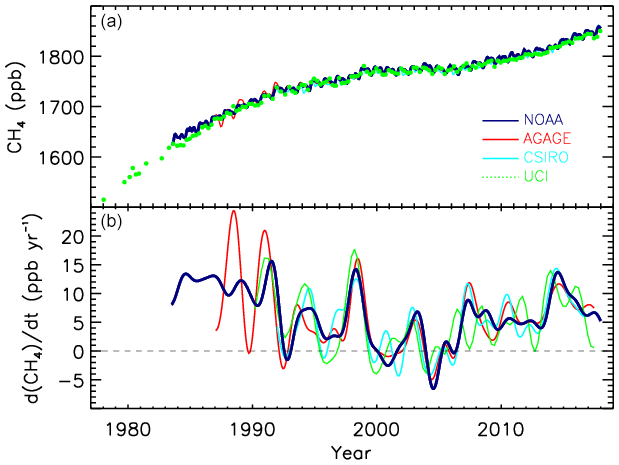
\includegraphics[width=0.6\textwidth]{Images/ch4_trend.png}
    \caption[Global \ch{CH_4} trends from 1983 to 2025]{Globally-averaged atmospheric \ch{CH_4} concentrations at Earth's surface (monthly means, red curve) and long-term trend (black curve). Methane has climbed from approximately 1630~ppb in 1983 to around 1930~ppb in 2025, with a notable stabilization in the early 2000s followed by a sharp rise in the past decade. The seasonal cycle (red oscillations) is driven by variations in OH sink and source seasonality. Data source: NOAA Global Monitoring Laboratory (after Dlugokencky et al., 1994 and updates) \cite{Saunois2020}.}
    \label{fig:ch4_global_trend}
\end{figure}

Against this background, satellite observations provide the essential evidence base for disentangling methane variability and attributing it to sources and processes. A core dataset for this study is the atmospheric methane observations from the TROPOspheric Monitoring Instrument (TROPOMI) aboard ESA's Sentinel-5 Precursor satellite. TROPOMI provides near-daily global measurements of column-averaged methane (XCH$_4$) at high spatial resolution (initially $\sim$7$\times$7 km$^2$, improved to 5.5$\times$7 km$^2$ in mid-2019) \cite{Hu2016, Lorente2021}. These data enable detection of regional enhancements and temporal variability. The operational retrieval algorithm uses SWIR spectral bands to infer XCH$_4$ \cite{Hu2016}, with subsequent updates improving bias corrections \cite{Lorente2021}.

Ground-based networks complement satellite observations by providing high-precision, continuous measurements for validation and long-term trend analysis. The NOAA Global Monitoring Laboratory operates a comprehensive network of flask sampling and in-situ measurement sites worldwide, delivering the foundational record shown in Figure~\ref{fig:ch4_global_trend} \cite{Dlugokencky2011}. The Total Carbon Column Observing Network (TCCON) provides ground-based Fourier Transform Spectrometer measurements of column-averaged dry-air mole fractions, offering independent validation of satellite retrievals with precision better than 0.25\% \cite{Wunch2011}. These networks are crucial for bias correction of satellite data and for understanding the representativeness of space-based observations across different spatial and temporal scales.

Earlier missions such as JAXA's GOSAT offered longer-term records at coarser resolution \cite{Parker2018}, but TROPOMI's finer detail enables attribution of emissions to specific surface characteristics \cite{Pandey2021, Zhang2020}. Applications already span wetland flux estimation, detection of large point sources, and inversion-based budget constraints \cite{Pandey2021, Zhang2020, Maasakkers2019}, demonstrating its value for causal time-series analysis.

Auxiliary datasets are essential for attribution. Meteorological data including wind fields, temperature, and pressure from reanalyses such as ERA5 \cite{Hersbach2020} provide critical forcing variables that influence methane production, transport, and oxidation processes. Wind patterns control atmospheric transport and mixing, while temperature and soil moisture directly affect microbial methane production in wetlands and agricultural soils. These factors explain anomalies such as East African wetland pulses \cite{Lunt2021} or ENSO-linked variability \cite{Parker2018}. 

Emission inventories complement observations by providing spatially explicit estimates of anthropogenic and natural sources. EDGAR provides comprehensive global inventories of anthropogenic methane emissions by sector \cite{Crippa2020}, while the EPA maintains detailed national inventories with facility-level data for major emitting countries. For natural sources, WetCHARTs delivers process-based wetland emission estimates \cite{Bloom2017}, incorporating biogeochemical modeling with satellite-derived inundation maps.

Land use and socio-economic data provide additional context for understanding emission patterns and their drivers. MODIS land cover \cite{Friedl2010} provides annual classification of wetlands, agriculture, and forests at 500 m--1 km resolution; ESA WorldCover delivers 10 m resolution updates \cite{Lorente2021}. Socio-economic indicators including population density, livestock numbers, rice cultivation areas, and energy production statistics enable attribution of methane variability to specific human activities and natural processes.

Top-down inversions often adjust these bottom-up priors \cite{Maasakkers2019, Saunois2020}, showing the complementarity of datasets and the importance of integrating multiple observation types and modeling approaches.

In summary, the observational basis of this study consists of time series of TROPOMI methane, augmented by ground-based networks (NOAA, TCCON), meteorological data (wind, temperature, pressure), emission inventories (EDGAR, EPA), and land use and socioeconomic data. This ensemble enables causal machine learning to disentangle the natural and anthropogenic drivers of methane variability, ensuring that the results are both statistically robust and physically interpretable.

Although the preceding discussion has outlined the broad spectrum of observational data supporting methane research, the technical aspects of satellite-based methane retrievals deserve a detailed examination given their central role in this study. The following subsection delves into the specific methodologies, algorithms, and challenges associated with remote sensing of atmospheric methane, providing a foundation for understanding how space-based observations are transformed into scientifically useful data sets for causal analysis.

\subsection{Satellite-Based Methane Retrievals and Remote Sensing}
\label{sec:satellite-retrievals}

Satellite instruments such as TROPOMI (aboard Sentinel-5P) and GOSAT have significantly advanced global methane monitoring by enabling frequent high-resolution observations of column-averaged methane concentrations (XCH\textsubscript{4}) \cite{Schneising2019, Lorente2021}. Spaceborne remote sensing has become a cornerstone of atmospheric methane (\ch{CH_4}) monitoring, enabling global, high-resolution observation of methane concentrations and emission dynamics. Satellite-based systems allow systematic tracking of both diffuse and concentrated sources across temporal and spatial scales that are unattainable by surface-based or airborne networks alone. They have been instrumental in detecting large emission events, characterizing seasonal and interannual variability, and supporting verification of mitigation targets \cite{eo_portal_iss_2023, ghgsat_ghgsat_2023, writer_methane_tracking_2023}.

Historically, atmospheric \ch{CH_4} observations relied on sparse ground stations and aircraft campaigns. The advent of satellite instruments capable of detecting methane via shortwave-infrared (\gls{swir}) spectroscopy has since transformed this field by retrieving the column-averaged dry-air mole fraction (\gls{xch4}) from sunlight reflected off Earth's surface and scattered through the atmosphere \cite{Karoff2023}. Atmospheric methane can be measured from space by observing solar radiation in SWIR bands absorbed by CH$_4$ in the atmospheric column.

Among these, the TROPOMI/WFMD product, developed at the University of Bremen, has played a central role due to its near-daily global coverage, systematic quality control, and robust uncertainty estimates \cite{Schneising2019}. Two major retrieval algorithms have been used to generate methane concentrations from TROPOMI radiance measurements: the Weighting Function Modified Differential Optical Absorption Spectroscopy (WFM-DOAS) and RemoTeC. WFM-DOAS, initially developed for SCIAMACHY, has been adapted for TROPOMI as a computationally efficient method. It emphasizes spectroscopic fitting speed and has benefited from recent refinements that reduce biases in XCH\textsubscript{4} and XCO. RemoTeC, in contrast, implements a full-physics optimal estimation framework that explicitly accounts for cloud and aerosol scattering through iterative radiative transfer simulations \cite{evaluation}. It employs Tikhonov regularization for vertical profile retrievals and draws on heritage from GOSAT and OCO-2 retrievals. As of now, RemoTeC serves as the operational Level 2 retrieval algorithm for Sentinel-5P methane products.

The complementary design of these retrieval strategies allows for comparative analysis of algorithmic uncertainties. Karoff and Vara-Vela \cite{Karoff2023}, for example, combined outputs from both methods to ensure robustness in their identification of spatial and seasonal methane patterns. Such dual-use approaches help to mitigate retrieval-specific artifacts that may otherwise distort atmospheric interpretation.

\subsubsection{Satellite Mission Capabilities and Limitations}

Over the past two decades, an array of satellite missions has been deployed to monitor methane, each with distinct spatial resolution, coverage, and spectral characteristics. Table~\ref{tab:missions} summarizes key current satellite missions for atmospheric CH$_4$ monitoring, including their operators, launch dates, spatial/temporal resolution, coverage, and notable features.

\begin{longtable}{l l c p{2.2cm} p{2.1cm}}
\caption{\parbox{0.8\linewidth}{Key satellite missions for atmospheric methane monitoring. Attributes include operator, launch date, spatial resolution, and revisit/coverage.}}
\label{tab:missions} \\
\hline
\textbf{Mission} & \textbf{Operator} & \textbf{Launch} & \textbf{Resolution} & \textbf{Revisit} \\
\hline
\endfirsthead
\caption[]{\parbox{\linewidth}{(Continued from previous page)}}\\
\hline
\textbf{Mission} & \textbf{Operator} & \textbf{Launch} & \textbf{Resolution} & \textbf{Revisit} \\
\hline
\endhead
GOSAT-2$^{\dagger}$ & JAXA (Japan) & 2018 & $\sim$10 km & 3-day (sampling) \\
TROPOMI (S5P)$^{\ddagger}$ & ESA/KNMI & 2017 & 7×7 km & Daily global \\
GHGSat-C/D (Valmay)$^{\S}$ & GHGSat Inc. (Canada) & 2025 & $\sim$25 m & Tasked, on-demand \\
MethaneSAT$^{\P}$ & EDF / NZ Space Agency & 2024 & 100--400 m & 3--4 d \\
PRISMA & ASI (Italy) & 2019 & 30 m & $\sim$7 d \\
EnMAP & DLR (Germany) & 2022 & 30 m & $\sim$4 d \\
WorldView-3 & Maxar (USA) & 2014 & 3.7 m (SWIR) & On-demand \\
\hline
\multicolumn{5}{p{\linewidth}}{\footnotesize $^{\dagger}$ Successor to GOSAT (Ibuki, 2009).} \\
\multicolumn{5}{p{\linewidth}}{\footnotesize $^{\ddagger}$ Pixel size improved from 7×7 to 5.5×7 km$^2$ in 2019 (Lorente et al., 2021).} \\
\multicolumn{5}{p{\linewidth}}{\footnotesize $^{\S}$ GHGSat constellation includes D (Claire, 2016), Iris (C1, 2020), Hugo (C2, 2021), Luca/Penny/Diako (C3--C5, 2022), May-Lin/Gaspard/Océane (C6--C8, 2023), and Juba/Vanguard/Elliot (C9--C11, 2023).} \\
\multicolumn{5}{p{\linewidth}}{\footnotesize $^{\P}$ MethaneSAT launched March 2024; lost contact June 2025. Data collected before loss remain valuable.} \\
\end{longtable}

These missions fall broadly into two complementary classes \cite{Jacob2022}: (1) \textit{area flux mappers} with coarse (km-scale) pixels and high precision, designed for mapping regional to global methane distributions, and (2) \textit{point-source imagers} with fine (meter-scale to tens of meters) pixels, capable of resolving individual methane plumes from strong localized emitters. The synergistic use of these satellites enables detection of both diffuse, widespread emissions and concentrated point sources of methane.

Launched in 2009 by JAXA, the Greenhouse Gases Observing Satellite (GOSAT) was the first dedicated greenhouse gas mission. Provides a calibration-grade record of \ch{XCH4} that has been widely used in top-down inversion studies \cite{Parker2020, Jacob2022}. Despite its importance for establishing long-term global trends, its sparse spatial coverage and coarse footprint limit its ability to resolve localized methane plumes.

The launch of ESA's TROPOMI aboard Sentinel-5P in 2017 revolutionized methane monitoring by offering daily global coverage at moderate spatial resolution. TROPOMI has revealed numerous ultra-emitters \cite{Pandey2019, Lauvaux2022}, significantly advancing the detection of large emission events. Nevertheless, its coarse pixels dilute concentrated plumes and retrievals are often hindered by persistent cloud cover or low surface reflectivity, particularly in tropical regions \cite{Jacob2022, Lorente2021}.

Complementing these flux mappers, the commercial GHGSat constellation provides facility-scale imaging with a ground sampling distance of approximately 25 m. It is capable of detecting sustained leaks of a few hundred kilograms of methane per hour under favorable conditions \cite{Varon2019, Varon2020}. However, GHGSat satellites must be specifically tasked to known sites, and their sensitivity is strongly influenced by scene conditions, which constrains systematic monitoring.

MethaneSAT, scheduled for launch in 2024, is designed to bridge the gap between coarse mappers and high-resolution imagers. With a nominal pixel size of about 0.3 km, it will combine high precision with improved spatial detail, although its coverage will be restricted to selected high-emission domains \cite{Jacob2022}. By doing so, it aims to enable basin-scale flux quantification while still detecting point sources that are beyond TROPOMI's detection capability.

In parallel, hyperspectral missions such as PRISMA (launched in 2019) and EnMAP (launched in 2022) have demonstrated the ability to detect methane plumes at 30 m resolution \cite{Guanter2021, Sherwin2024}. While their acquisitions are tasked and therefore sparse, they provide confirmatory information on hotspots flagged by wide-swath sensors, adding confidence and spatial detail to emission source identification.

At the very high-resolution end of the spectrum, Maxar's WorldView-3 provides sub-4 m sensitivity in SWIR bands, enabling detection of methane plumes as small as 90 kg,h$^{-1}$ \cite{Sanchez2022}. Its ultra-fine spatial detail allows direct attribution of emissions to specific facilities or infrastructure. However, the presence of only a single CH$_4$-absorbing band and the high cost of tasked acquisitions limit its quantitative reliability and systematic use.

Looking ahead, the planned CarbonMapper constellation will expand systematic hyperspectral coverage at 30 m resolution with open data access, targeting urban, industrial, and agricultural hotspots. Additional forthcoming missions, including Sentinel-5 (post-2025) and GOSAT-GW, will extend the mapper record with improved precision, while the Franco-German MERLIN lidar mission (expected by 2027) will pioneer active sensing to detect methane under conditions where passive sensors fail, such as polar night or thin cloud cover.

\subsubsection{Retrieval Limitations and Challenges}

Notwithstanding these advances, satellite-based methane retrievals remain subject to several critical limitations. One persistent challenge involves surface reflectance effects: scenes with either very low (e.g., densely vegetated wetlands, water bodies) or very high albedo (e.g., snow, ice, deserts) can induce systematic retrieval errors in XCH\textsubscript{4} \cite{Lorente2021}. While bias correction schemes have substantially improved performance, residual discrepancies persist in extreme surface conditions. Additional uncertainty arises from clouds and aerosols. Even with stringent cloud filtering, subvisual clouds or aerosol layers can introduce scattering-induced distortions. RemoTeC attempts to correct for this by jointly retrieving aerosol properties, but uncertainties remain, particularly in partially cloud-contaminated scenes.

A more fundamental limitation stems from the nature of the retrieval: TROPOMI measures total column concentrations, which integrate emission sources, transport, and chemical sinks. Without supporting models, it is difficult to attribute observed anomalies exclusively to surface-level emissions. This complicates the separation of emission-driven signals from those arising due to vertical mixing, advection, or oxidation.

These limitations are not merely theoretical. Karoff and Vara-Vela \cite{Karoff2023} documented anomalously low methane concentrations over known wetland regions---an unexpected outcome given that wetlands are among the strongest natural emitters of methane. This finding suggests the presence of retrieval artifacts, likely related to the interaction of water surfaces, high humidity, and atmospheric scattering in retrieval algorithms. Such examples highlight the importance of robust analytical tools capable of accounting for these confounding influences.

\subsubsection{Satellite Applications and Achievements}

Despite these challenges, TROPOMI and related instruments have demonstrated substantial value in global methane monitoring. Pandey et al. \cite{Pandey2017} used GOSAT and supporting data to detect a 6--9~Tg/yr increase in wetland methane emissions during the 2011 La Niña. Their work demonstrated the sensitivity of satellite-based retrievals to large-scale hydrological variability. Similarly, Jodhani et al. \cite{Jodhani2024} combined TROPOMI methane data with MODIS and Landsat land cover products to investigate pollutant distributions in western India. They found that while species like \ch{NO_2} and \ch{CO} showed localized hotspots over industrial areas, methane displayed more uniform spatial patterns due to its longer atmospheric lifetime and broader sources.

Consistent spatial gradients in XCH\textsubscript{4} concentrations have also been observed across ecosystems. High values frequently occur over regions of intensive agriculture, livestock production, and fossil fuel extraction. In contrast, lower values are typically associated with arid or sparsely vegetated landscapes with minimal methane fluxes. These observations align with known emission patterns and reinforce the interpretability of satellite-derived methane products.

\subsection{Auxiliary Data and Contextual Information}

Ancillary datasets further support attribution. TROPOMI retrieves \(\mathrm{XCO}\) alongside \(\mathrm{XCH_4}\). MODIS (Terra/Aqua) provides land cover (MCD12Q1), aerosol optical depth (AOD), vegetation indices, and fire detections at 500 m resolution, while ESA WorldCover provides 10 m global land cover \cite{Karoff2023}. Table~\ref{tab:contextual_products} summarizes these contextual products.

\begin{table}[htbp]
\centering
\caption{Earth observation missions supporting methane monitoring through land-cover and environmental context.}
\label{tab:contextual_products}
\small
\begin{tabularx}{\textwidth}{@{}l l c c X@{}}
\toprule
\textbf{Mission/Product} & \textbf{Operator} & \textbf{Launch} & \textbf{Res.} & \textbf{Use and Limitations} \\
\midrule
MODIS (Terra \& Aqua) & NASA & 1999, 2002 & 500 m & Provides land cover (MCD12Q1), aerosol optical depth (AOD), vegetation indices, and fire detection; mixed-pixel issues in heterogeneous terrain. \\
ESA WorldCover & ESA & 2021 & 10 m & High-resolution annual global land cover maps; valuable for masking and classification; short record, validation ongoing. \\
\bottomrule
\end{tabularx}
\end{table}

Building upon these advancements, this research leverages enhanced TROPOMI products (WFMD, S5P-RemoTeC) with improved albedo corrections, filtering, and cloud masking \cite{rajnauth_monetizing_2008}. Integrated with MODIS-derived land cover and AOD in the \gls{gee} platform \cite{Gorelick2017}, this forms a multi-dimensional dataset essential for spatiotemporal exploration of methane drivers.

This thesis builds upon these advances by leveraging the TROPOMI WFM-DOAS product alongside MODIS and Sentinel-2 land cover datasets. While retrieval biases and structural limitations persist, they can be mitigated through quality screening, stratification by surface type, and causal methods that explicitly model confounding factors. The methodological procedures described in Chapter~\ref{chap:methodology} incorporate these corrections to enable interpretable and statistically valid inference over diverse regions and time scales.

However, disentangling true drivers from spurious co-variations requires moving beyond statistical associations to rigorous causal inference. For example, an anomalous surge in XCH$_4$ over the tropics might suggest wetter-than-usual wetlands or reduced OH in that period, whereas a steep decline in spring methane corresponds to enhanced OH-driven loss. In a causal modeling framework, incorporating knowledge of these processes, such as the sensitivity of wetland emissions to climate oscillations or the role of transport in spreading anthropogenic plumes, is crucial for correctly attributing observed methane variations to their drivers. The literature provides a rich foundation of process understanding to inform such models, ensuring that statistical inferences from satellite time series are physically plausible and grounded in the known methane cycle.

%%%%%%%%%%



% New structure: 
%\chapter{Introduction}

%       \subsection{Patterns, Dependencies, and Relationships in Observations}
%           \subsubsection{Statistical Methods for Dependency Analysis}
%           \subsubsection{Correlation and Its Interpretive Limits}
%           \subsubsection{Visual and Mathematical Comparison}

%       \subsection{Foundations of Causality}
%           \subsubsection{From Association to Explanation: The Need for Causal Analysis}
%           \subsubsection{Causal Inference vs. Statistical Learning}
%               Statistical learning models associations: \( P(Y \mid X) \) \\
%               Causal inference models interventions: \( P(Y \mid \text{do}(X)) \)

%           \subsubsection{Pearl's Causal Hierarchy}
%               \begin{itemize}
%                   \item Level 1: Associational ,  Seeing ,  Do methane levels correlate with temperature?
%                   \item Level 2: Interventional ,  Doing ,  What happens to methane if we reduce emissions?
%                   \item Level 3: Counterfactual ,  Imagining ,  Would methane have decreased if a policy had been enacted earlier?
%                   \end{itemize}
            
%           \subsubsection{Structural Causal Models (SCMs)}
%               Defined as: \( M = \langle U, V, F, P(U) \rangle \)

%           \subsubsection{Integrating Land Cover and Atmospheric Constituents}

%           \subsubsection{Motivation for a New Causal-Guided Framework}





% TODO:
% Add this subsection: Statistical Properties of Methane Series and these subsubsections:
% Seasonal cycles, interannual variability, long-term trends
% Spatial autocorrelation across regions

\section{Patterns, Dependencies, and Relationships in Observations}

Understanding atmospheric methane dynamics requires sophisticated approaches to identify meaningful relationships within complex, high-dimensional observational datasets. Before establishing causal frameworks, it is essential to recognize the fundamental distinction between observable patterns, statistical dependencies, and genuine causal relationships. This distinction becomes particularly crucial when analyzing Earth system data, where multiple interacting processes operate across different spatial and temporal scales, creating intricate webs of apparent associations that may or may not reflect underlying causal mechanisms.

The challenge of interpreting observational patterns in atmospheric methane research exemplifies broader issues in Earth system science. Satellite observations of methane concentrations, ground-based measurements, and ancillary environmental data collectively generate vast datasets where correlations abound, yet distinguishing meaningful relationships from spurious associations remains non-trivial. As \cite{Runge2019} emphasizes, the complexity of Earth system interactions demands rigorous statistical frameworks that can separate genuine dependencies from coincidental patterns arising from common drivers, confounding variables, or temporal autocorrelation.

Traditional approaches to pattern recognition in environmental sciences have relied heavily on correlation analysis, regression modeling, and spectral decomposition techniques. While these methods provide valuable insights into data structure and variability, they are fundamentally limited in their capacity to distinguish between different types of relationships. A high correlation between methane concentrations and temperature, for instance, might reflect direct causal influence, shared response to a common driver such as seasonal cycles, or purely coincidental temporal alignment. Without additional analytical frameworks, correlation-based approaches cannot resolve these ambiguities, potentially leading to misattribution of environmental processes and ineffective policy interventions.

\subsection{Statistical Methods for Dependency Analysis}

Contemporary statistical methods for analyzing dependencies in environmental data encompass a broad spectrum of techniques, each with distinct assumptions, capabilities, and limitations. Linear correlation analysis, while ubiquitous in environmental research, represents only the simplest form of dependency detection. Pearson correlation coefficients capture linear relationships between variables but are fundamentally inadequate for detecting nonlinear associations, temporal delays, or directional dependencies that characterize many Earth system processes \cite{Kraskov2004}.

Information-theoretic approaches offer more sophisticated alternatives for dependency analysis in complex systems. Mutual information, originally developed in communication theory, quantifies the reduction in uncertainty about one variable given knowledge of another, regardless of the functional form of their relationship \cite{Kraskov2004}. This property makes mutual information particularly valuable for analyzing environmental datasets where relationships may be highly nonlinear, as is common in biogeochemical cycles and atmospheric chemistry. For methane research, mutual information can reveal dependencies between emissions and environmental drivers that linear methods might miss, such as threshold effects in wetland productivity or nonlinear responses to temperature variations.

Transfer entropy extends information-theoretic analysis to capture directional dependencies and temporal relationships \cite{Schreiber2000}. Unlike symmetric measures such as correlation or mutual information, transfer entropy quantifies the information flow from one time series to another, providing insights into the direction and magnitude of statistical influence. Recent applications in climate science have demonstrated the utility of transfer entropy for identifying drivers of extreme events and understanding feedback mechanisms in coupled Earth system components \cite{Palus2024, li_integrating_2025}.

Advanced spectral methods provide complementary approaches for analyzing temporal dependencies in environmental time series. Cross-spectral analysis can reveal frequency-domain relationships between variables, identifying whether dependencies occur primarily at seasonal, interannual, or decadal timescales. For methane observations, spectral coherence analysis can distinguish between dependencies arising from seasonal biogeochemical cycles versus those driven by longer-term climate variability or anthropogenic trends \cite{tongal_forecasting_2021}.

Machine learning approaches have increasingly been applied to dependency analysis in Earth system science, offering powerful tools for detecting complex, high-dimensional relationships. Kernel-based methods can capture nonlinear dependencies while maintaining statistical rigor, and ensemble approaches can provide robust estimates of relationship strength across different model specifications \cite{Marinazzo2008}. However, these methods typically focus on predictive performance rather than interpretability, limiting their utility for understanding underlying mechanisms.

The choice among these analytical approaches depends critically on the specific research questions, data characteristics, and underlying assumptions about system behavior. Linear methods remain valuable for initial exploratory analysis and for systems where linear approximations are reasonable. Information-theoretic methods excel in situations where relationships may be highly nonlinear or where distributional assumptions are difficult to justify. Spectral methods are particularly powerful for analyzing cyclical processes and distinguishing between different timescales of variability.




\subsection{Correlation and Its Interpretive Limits}

Correlation analysis remains the most widely used method for quantifying relationships in environmental datasets, yet its interpretive limitations are frequently underappreciated in applied research. The fundamental challenge lies in the multiple mechanisms that can generate correlation between variables, only some of which reflect meaningful dependencies relevant to scientific understanding or policy applications.

Spurious correlation represents perhaps the most significant interpretive pitfall in environmental data analysis. When two variables exhibit temporal trends, statistical correlation can arise purely from their shared trend components, even when no direct relationship exists between the underlying processes. This phenomenon is particularly problematic in climate and atmospheric research, where many variables exhibit long-term trends due to anthropogenic forcing or natural climate variability. For methane research, apparent correlations between emissions and various environmental drivers may reflect common responses to climate change rather than direct causal relationships.

Common cause confounding presents another critical limitation of correlation-based analysis. When two variables are influenced by the same underlying driver, they may exhibit strong correlation despite having no direct relationship. In methane studies, correlations between wetland emissions and temperature might actually reflect their shared dependence on broader climate patterns, soil moisture availability, or seasonal phenological cycles. Distinguishing between direct relationships and common cause scenarios requires careful consideration of potential confounding variables and appropriate statistical control methods.

Temporal autocorrelation in environmental time series further complicates correlation interpretation. When variables exhibit persistence or memory effects, correlations can be inflated by the autocorrelation structure rather than reflecting genuine cross-variable relationships. This issue is particularly acute in atmospheric observations, where transport processes create spatial and temporal dependencies that can generate misleading correlation patterns \cite{attanasio2013}.

The directionality ambiguity inherent in correlation measures represents another fundamental limitation. Even when correlation reflects genuine dependency rather than spurious association or confounding, symmetric correlation coefficients provide no information about the direction of influence. For policy-relevant applications, understanding whether methane concentrations drive environmental responses or vice versa is crucial for designing effective interventions.

Scale dependence adds additional complexity to correlation interpretation in Earth system applications. Relationships between variables may vary substantially across different temporal or spatial scales, with correlations that are strong at one scale potentially being weak or absent at others. Methane emissions may correlate strongly with temperature at daily timescales due to direct biochemical effects, while showing weaker or different relationships at seasonal or interannual scales where ecosystem adaptation and human responses become important.

Statistical significance testing, while standard practice in correlation analysis, provides limited guidance for scientific interpretation. High statistical significance can occur for very weak correlations in large datasets, while scientifically meaningful relationships may fail to achieve conventional significance thresholds due to measurement noise, sampling limitations, or natural variability. The focus on statistical rather than practical significance can mislead researchers about the importance of observed relationships.




\subsection{Visual and Mathematical Comparison}

Effective analysis of dependencies in environmental datasets requires integration of visual exploration and mathematical quantification, as each approach reveals different aspects of complex relationships. Visual methods excel at revealing data structure, identifying outliers, and suggesting appropriate analytical approaches, while mathematical measures provide precise quantification and statistical inference capabilities.

Scatterplot analysis remains fundamental for understanding bivariate relationships, yet its effectiveness depends critically on appropriate data preparation and visualization choices. For environmental time series, simple X-Y plots may obscure important temporal patterns or cyclical relationships. Phase space reconstructions and lag plots can reveal temporal dependencies and nonlinear dynamics that are invisible in traditional scatterplots. For methane observations, plotting concentration anomalies against environmental drivers at various temporal lags can reveal both instantaneous and delayed responses that inform mechanistic understanding.

Time series visualization presents unique challenges and opportunities for dependency analysis. Overlaying multiple variables on common time axes can reveal coincident patterns and suggest potential relationships, but differences in scales and units often necessitate normalization or transformation. Wavelet analysis and time-frequency representations can reveal how relationships vary across different timescales, identifying whether dependencies are consistent or episodic \cite{tongal_forecasting_2021}.

Correlation matrices and heatmaps provide comprehensive overviews of relationships within multivariate datasets, enabling identification of variable clusters and potential redundancies. For high-dimensional environmental datasets, hierarchical clustering of correlation matrices can reveal underlying data structure and guide variable selection for more detailed analysis. However, correlation matrices can be misleading when relationships are nonlinear or when temporal dependencies are important.

Network visualization approaches represent an emerging frontier for analyzing complex environmental dependencies. By representing variables as nodes and relationships as edges, network diagrams can reveal system-level patterns of connectivity and identify key variables that mediate relationships between different components. Recent applications in climate science have used network approaches to identify teleconnections and critical transition points in coupled Earth system components \cite{Runge2019}.

Mathematical comparison of different dependency measures provides essential validation for visual insights and enables rigorous hypothesis testing. Comparative analysis of linear correlation, rank correlation, mutual information, and transfer entropy for the same variable pairs can reveal the nature and strength of relationships while identifying potential nonlinearities or directional asymmetries. For methane research, such comparative analysis might reveal that temperature-emission relationships are stronger when quantified using information-theoretic measures rather than linear correlation, suggesting important nonlinear threshold effects.

Bootstrap resampling and permutation testing provide robust approaches for assessing the statistical significance and stability of observed relationships. These methods are particularly valuable for environmental applications where distributional assumptions may be violated and where temporal dependencies complicate traditional significance testing. Confidence intervals derived from bootstrap methods can quantify uncertainty in relationship estimates and guide interpretation of observed patterns.

Cross-validation approaches enable assessment of relationship stability and generalizability across different time periods or spatial domains. For methane observations, split-sample validation can reveal whether relationships observed during specific periods are representative of longer-term system behavior or reflect particular climatological conditions.

The integration of visual and mathematical approaches is particularly powerful for identifying data quality issues, measurement artifacts, and analytical assumptions. Visual inspection can reveal outliers, non-stationarities, and distributional departures that might compromise mathematical analyses, while quantitative measures can confirm or refute apparent visual patterns. This iterative approach between exploration and quantification represents best practice for dependency analysis in complex environmental systems.

Ultimately, the combination of sophisticated statistical methods, careful attention to interpretive limitations, and integrated visual-mathematical approaches provides the foundation for moving beyond simple pattern recognition toward genuine understanding of system dependencies. This foundation is essential for subsequent causal analysis, where the goal shifts from describing relationships to understanding the mechanisms that generate them.



%%%%%%%%%%%%%%%%%%%%%%%%%%%%%%%%%%%%%%%%
\section{The Role of Causal Analysis}
\label{sec:causal_analysis}

Understanding the mechanisms that drive atmospheric methane (\ch{CH_4}) dynamics requires analytical approaches that transcend traditional statistical methods. While correlation-based techniques have long served as the foundation for analyzing environmental data, they fundamentally cannot distinguish between genuine cause-effect relationships and spurious associations arising from confounding variables, reverse causation, or mere coincidence. In the context of satellite-based methane monitoring, this limitation becomes particularly acute: observed correlations between methane concentrations and surface temperature might reflect direct causal influence, reverse causation, or both variables responding to unmeasured drivers such as soil moisture or microbial activity \cite{triacca_is_2005}.

The need for causal understanding extends beyond academic curiosity to practical necessity. Policy interventions aimed at reducing methane emissions require knowledge of causal mechanisms, not merely statistical associations. Predicting system responses to climate change demands understanding of feedback loops and tipping points that correlation alone cannot reveal. Attribution of observed methane increases to specific sources, whether natural wetlands, agricultural practices, or fossil fuel operations, necessitates causal reasoning that can separate direct effects from indirect correlations \cite{Saunois2020}.

This section establishes the theoretical foundations and practical methodologies of causal analysis as applied to environmental monitoring systems. We begin by distinguishing causal inference from statistical learning, introducing Pearl's causal hierarchy that formalizes different levels of causal reasoning. We then develop the mathematical framework of structural causal models and their graphical representations, which provide both intuitive visualization and rigorous inference tools. The discussion progresses to causal discovery methods for both static and temporal data, with particular emphasis on time series approaches relevant to satellite observations. Throughout, we maintain focus on methane as our target variable, illustrating how these methods transform satellite data from descriptive measurements to mechanistic understanding of Earth system processes.

\subsection{From Association to Explanation}

The journey from observing patterns to understanding mechanisms represents a fundamental shift in scientific reasoning. Statistical associations, while valuable for pattern recognition and prediction, reveal what happens together but not why. Consider the seasonal correlation between rice paddy extent and atmospheric methane concentrations observed in satellite data. This correlation might suggest that rice cultivation drives methane emissions, a plausible hypothesis given that flooded rice fields create anaerobic conditions favorable to methanogenesis. However, the correlation could equally arise from both variables responding to monsoon seasonality, with rainfall simultaneously enabling rice cultivation and enhancing natural wetland emissions \cite{patra2016}.

This ambiguity pervades environmental systems where multiple processes interact across scales. Temperature correlates with methane emissions, but does warming directly enhance microbial methanogenesis, or does it act indirectly by extending wetland area, increasing substrate availability, or altering plant productivity? Does elevated atmospheric methane contribute to warming through radiative forcing, creating a positive feedback loop? Statistical correlation cannot answer these questions because it captures symmetric relationships: if X correlates with Y, then Y correlates with X to the same degree.

Causal analysis breaks this symmetry by distinguishing causes from effects. It recognizes that intervening to change X may alter Y, while intervening on Y might leave X unchanged. This asymmetry reflects the fundamental arrow of causation in physical systems. When we drain a wetland, methane emissions decrease; when we remove methane from the atmosphere, wetlands do not disappear. This directional relationship, invisible to correlation, becomes explicit through causal analysis.

The transition from association to causation requires three conceptual advances. First, we must formalize what we mean by causation, moving from intuitive notions to mathematical definitions. Second, we need frameworks to represent causal relationships, typically through directed graphs that encode our assumptions about system structure. Third, we require methods to infer causal relationships from data, either testing specific causal hypotheses or discovering causal structure from observations.

\begin{table}[h!]
\centering
\caption{Comparison of Association and Causation in Methane Systems}
\label{tab:association_vs_causation}
\begin{tabular}{p{3cm}|p{6cm}|p{6cm}}
\hline
\textbf{Aspect} & \textbf{Association} & \textbf{Causation} \\
\hline
\textbf{Question Type} & What patterns exist in the data? & What mechanisms generate the patterns? \\
\textbf{Symmetry} & Symmetric: X correlates with Y implies Y correlates with X & Asymmetric: X causes Y does not imply Y causes X \\
\textbf{Prediction} & Under observed conditions & Under interventions and counterfactuals \\
\textbf{Example Query} & Do high temperatures coincide with high CH$_4$? & Does increasing temperature cause higher CH$_4$ emissions? \\
\textbf{Policy Relevance} & Limited, describes current state & Direct, predicts intervention outcomes \\
\textbf{Math Framework} & Joint distributions P(X,Y) & Structural equations and do-calculus \\
\textbf{Confounding} & Cannot detect or correct & Can identify and adjust for \\
\hline
\end{tabular}
\end{table}

The practical importance of this distinction becomes clear when designing monitoring systems and interventions. Association-based models might accurately predict methane concentrations from satellite-observed surface properties under current conditions. However, they fail when conditions change, through climate shifts, land-use modifications, or policy interventions, because they capture correlations specific to the observed data distribution rather than invariant causal mechanisms.

\subsection{Causal Inference versus Statistical Learning}

Statistical learning and causal inference represent fundamentally different paradigms for understanding data, each with distinct goals, methods, and limitations. This distinction, often underappreciated in applied sciences, becomes crucial when moving from pattern recognition to mechanistic understanding of environmental systems.

\subsubsection{The Statistical Learning Paradigm}

Statistical learning focuses on discovering patterns in data to optimize prediction accuracy. Given features X and outcome Y, statistical learning seeks the function $f$ that minimizes expected prediction error:
\begin{equation}
\hat{f} = \arg\min_f \mathbb{E}[(Y - f(X))^2]
\end{equation}

This optimization problem drives modern machine learning, from linear regression to deep neural networks. The resulting model captures the conditional distribution $P(Y|X)$, enabling prediction of Y given observations of X. Success is measured by predictive accuracy on held-out data, with techniques like cross-validation ensuring generalization to new observations from the same distribution.

In methane monitoring, statistical learning excels at tasks like predicting concentrations from satellite-observed surface properties, interpolating measurements across space and time, or detecting anomalous emission events. A deep learning model trained on TROPOMI observations might achieve remarkable accuracy in predicting methane concentrations from temperature, vegetation indices, and land cover. The model learns complex nonlinear relationships, automatically discovering predictive patterns without requiring explicit specification of functional forms.

However, this predictive capability comes with fundamental limitations. The model captures correlations specific to the training distribution, if trained on data from temperate regions, it may fail in the Arctic where different processes dominate. More fundamentally, it cannot answer causal questions: will reducing agricultural intensity decrease methane emissions? How would emissions respond to wetland restoration? What fraction of observed methane increase is attributable to anthropogenic versus natural sources?

\subsubsection{The Causal Inference Paradigm}

Causal inference seeks to understand the mechanisms generating observed data, focusing on how systems respond to interventions. Rather than modeling $P(Y|X)$, causal inference targets the interventional distribution $P(Y|\text{do}(X))$, where the do-operator represents external manipulation rather than passive observation.

This shift from observation to intervention fundamentally changes the inference problem. Consider the relationship between wetland extent and methane emissions. Statistical learning captures their correlation in observed data, where both may be driven by precipitation patterns. Causal inference asks: what would happen to methane emissions if we actively changed wetland extent through restoration or drainage? This interventional question cannot be answered from the observational distribution alone.

The mathematical distinction becomes clear when we consider confounding. Let Z represent precipitation, which affects both wetland extent (X) and methane emissions (Y). The observational distribution conflates the direct effect of X on Y with the spurious correlation induced by Z:
\begin{equation}
P(Y|X) = \sum_z P(Y|X,Z=z)P(Z|X)
\end{equation}

The interventional distribution removes the confounding by severing the link from Z to X:
\begin{equation}
P(Y|\text{do}(X)) = \sum_z P(Y|X,Z=z)P(Z)
\end{equation}

This adjustment formula, derived from causal assumptions encoded in a graphical model, isolates the causal effect of X on Y.

\begin{figure}[h!]
\centering
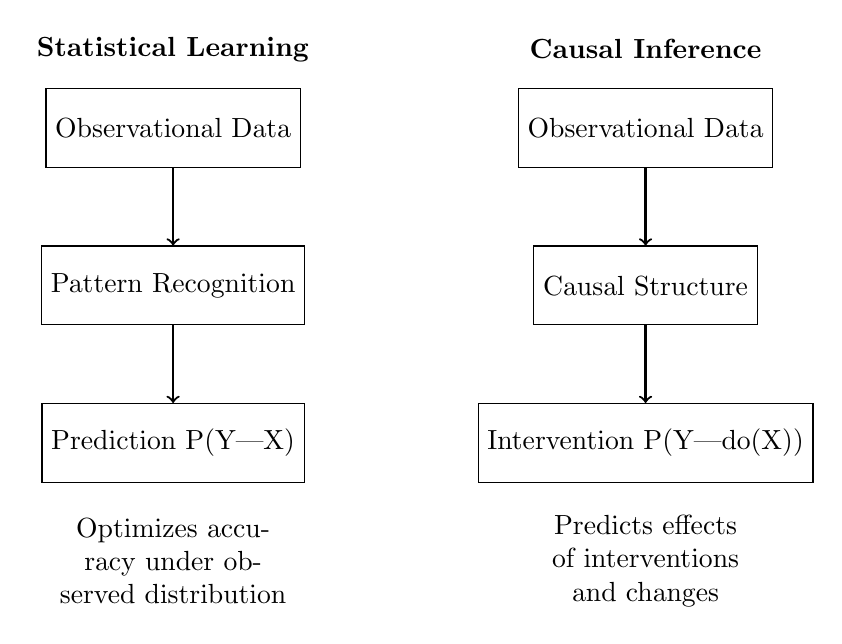
\begin{tikzpicture}[
   node distance=2cm,
   box/.style={rectangle, draw, minimum width=2.5cm, minimum height=1cm},
   arrow/.style={->, thick}
]
% Statistical Learning Side
\node[box] (data1) at (0,0) {Observational Data};
\node[box] (pattern) at (0,-2) {Pattern Recognition};
\node[box] (predict) at (0,-4) {Prediction P(Y|X)};

% Causal Inference Side
\node[box] (data2) at (6,0) {Observational Data};
\node[box] (struct) at (6,-2) {Causal Structure};
\node[box] (inter) at (6,-4) {Intervention P(Y|do(X))};

% Arrows for Statistical Learning
\draw[arrow] (data1) -- (pattern);
\draw[arrow] (pattern) -- (predict);

% Arrows for Causal Inference
\draw[arrow] (data2) -- (struct);
\draw[arrow] (struct) -- (inter);

% Labels
\node at (0,1) {\textbf{Statistical Learning}};
\node at (6,1) {\textbf{Causal Inference}};

% Annotations
\node[text width=3cm, align=center] at (0,-5.5) {Optimizes accuracy under observed distribution};
\node[text width=3cm, align=center] at (6,-5.5) {Predicts effects of interventions and changes};

\end{tikzpicture}
\caption{Contrasting paradigms: Statistical learning versus causal inference. While both begin with observational data, they diverge in goals and methods.}
\label{fig:paradigms}
\end{figure}

\subsubsection{When Each Paradigm Applies}

The choice between statistical learning and causal inference depends on the scientific question and intended application. Statistical learning suffices when:
\begin{itemize}
\item The goal is prediction under stable conditions
\item The data-generating process remains unchanged
\item We seek to detect patterns or anomalies
\item Interpolation or forecasting within observed ranges
\end{itemize}

Causal inference becomes necessary when:
\begin{itemize}
\item Evaluating potential interventions or policies
\item Attributing observed changes to specific causes
\item Predicting system response to unprecedented conditions
\item Understanding mechanisms and feedback loops
\item Generalizing across different contexts or populations
\end{itemize}

For comprehensive methane monitoring, both paradigms play complementary roles. Statistical learning enables real-time prediction and anomaly detection from satellite data. Causal inference reveals emission mechanisms, attributes sources, and predicts intervention outcomes. The integration of both approaches, using machine learning for pattern detection and causal methods for mechanistic understanding, provides the foundation for actionable environmental intelligence.

\subsection{Pearl's Causal Hierarchy}

Judea Pearl's causal hierarchy provides a formal taxonomy of causal reasoning, establishing three distinct levels of cognitive ability that cannot be reduced to one another \cite{Pearl2009}. This hierarchy, also known as the Ladder of Causation, demonstrates that different types of questions require fundamentally different types of information and inference machinery. Understanding this hierarchy is essential for recognizing what can and cannot be learned from different types of data and models.

\subsubsection{Level 1: Association (Seeing)}

The first level encompasses all questions answerable through statistical analysis of observational data. At this level, we ask about patterns, correlations, and conditional probabilities in the world as we observe it. The mathematical framework involves joint and conditional probability distributions derived from data.

Questions at this level take the form: "What is the probability of Y given that I observe X?" Formally:
\begin{equation}
P(Y|X) = \frac{P(X,Y)}{P(X)}
\end{equation}

In methane monitoring, Level 1 questions include:
\begin{itemize}
\item What is the correlation between temperature and methane concentrations?
\item Given current wetland extent, what methane levels do we expect?
\item How well can we predict emissions from observable surface properties?
\item What patterns exist in the seasonal cycle of atmospheric methane?
\end{itemize}

This level corresponds to most traditional statistical analysis and machine learning. Deep neural networks, despite their sophistication, operate entirely at Level 1, they discover complex patterns in observational data but cannot reason about interventions or counterfactuals. A model trained to predict methane from satellite imagery learns the observational distribution $P(\text{CH}_4|\text{imagery})$ but cannot answer what would happen if we changed the landscape.

The fundamental limitation of Level 1 is that it captures the world as it is, not as it could be under different circumstances. All patterns are specific to the observed data distribution. If that distribution changes, through climate shifts, policy interventions, or expansion to new regions, Level 1 models may fail catastrophically because they lack understanding of underlying causal mechanisms.

\subsubsection{Level 2: Intervention (Doing)}

The second level addresses questions about the effects of actions and interventions. Here we ask not what will happen given that we observe X, but what will happen if we deliberately set X to a specific value. This distinction, though subtle, is profound.

Questions at this level involve the do-operator: "What is the probability of Y if we intervene to set X to x?" Formally:
\begin{equation}
P(Y|\text{do}(X=x))
\end{equation}

This interventional distribution generally differs from the observational conditional distribution $P(Y|X=x)$ due to confounding. The do-operator represents a surgical modification of the system, we force X to take value x while leaving all other mechanisms unchanged.

In methane systems, Level 2 questions include:
\begin{itemize}
\item What will happen to emissions if we drain 10\% of wetlands?
\item How would atmospheric methane respond to eliminating fossil fuel extraction?
\item What is the effect of temperature increase on methane emissions?
\item Will changing agricultural practices reduce emissions?
\end{itemize}

These questions cannot be answered from observational data alone, no matter how much data we collect or how sophisticated our statistical methods. They require causal assumptions, typically encoded in structural causal models or directed acyclic graphs. With these assumptions, we can sometimes compute interventional distributions from observational data using techniques like the adjustment formula or instrumental variables.

\begin{figure}[h!]
\centering
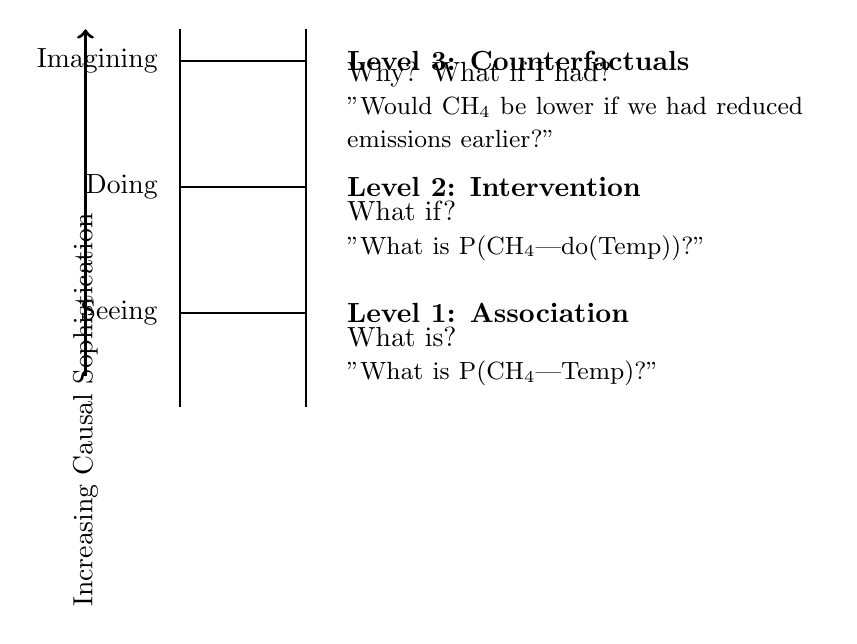
\begin{tikzpicture}[scale=0.8]
% Draw ladder
\draw[thick] (0,0) -- (0,6);
\draw[thick] (2,0) -- (2,6);

% Rungs
\draw[thick] (0,1.5) -- (2,1.5);
\draw[thick] (0,3.5) -- (2,3.5);
\draw[thick] (0,5.5) -- (2,5.5);

% Labels for levels
\node[right] at (2.5,1.5) {\textbf{Level 1: Association}};
\node[right] at (2.5,3.5) {\textbf{Level 2: Intervention}};
\node[right] at (2.5,5.5) {\textbf{Level 3: Counterfactuals}};

% Questions
\node[right, text width=6cm] at (2.5,0.8) {What is? \\
\small "What is P(CH$_4$|Temp)?"};
\node[right, text width=6cm] at (2.5,2.8) {What if? \\
\small "What is P(CH$_4$|do(Temp))?"};
\node[right, text width=6cm] at (2.5,4.8) {Why? What if I had? \\
\small "Would CH$_4$ be lower if we had reduced emissions earlier?"};

% Activity labels
\node[left] at (-0.2,1.5) {Seeing};
\node[left] at (-0.2,3.5) {Doing};
\node[left] at (-0.2,5.5) {Imagining};

% Arrow showing increasing capability
\draw[->, very thick] (-1.5,0.5) -- (-1.5,6) node[midway, left, rotate=90] {Increasing Causal Sophistication};

\end{tikzpicture}
\caption{Pearl's Causal Hierarchy: Three levels of causal reasoning, each requiring increasingly sophisticated inference machinery. Higher levels can answer questions from lower levels, but not vice versa.}
\label{fig:causal_hierarchy}
\end{figure}


The transition from Level 1 to Level 2 represents the difference between prediction and action. Climate models that forecast methane concentrations under current trends operate at Level 1. Policy analysis asking how emissions would change under specific interventions requires Level 2 reasoning.

\subsubsection{Level 3: Counterfactuals (Imagining)}

The third level encompasses counterfactual reasoning, questions about what would have happened in alternative scenarios that did not actually occur. These retrospective hypotheticals require the strongest form of causal reasoning.

Questions at this level ask: "Given that we observed X=x and Y=y, what would Y have been if X had been x'?" Formally:
\begin{equation}
P(Y_{x'}|X=x, Y=y)
\end{equation}

The notation $Y_{x'}$ represents the potential outcome, the value Y would have taken if X had been set to x'. This requires reasoning about individual cases, not just population distributions.

In methane analysis, Level 3 questions include:
\begin{itemize}
\item Would the 2020 methane spike have occurred without increased wetland extent?
\item What fraction of current atmospheric methane is attributable to anthropogenic sources?
\item Would Arctic emissions be lower today if warming had been prevented?
\item For a specific emission event, what would have happened under different weather conditions?
\end{itemize}

Counterfactual reasoning requires the strongest assumptions, we need fully specified structural equations, not just the causal graph. With these, we can compute counterfactuals through a three-step process:
\begin{enumerate}
\item \textbf{Abduction}: Infer the values of noise variables from observed data
\item \textbf{Action}: Modify the model to reflect the counterfactual intervention
\item \textbf{Prediction}: Compute outcomes under the modified model
\end{enumerate}

\subsubsection{The Hierarchy Theorem}

The Causal Hierarchy Theorem establishes that these three levels form a strict hierarchy, higher levels can answer questions from lower levels, but not vice versa. If we can compute counterfactuals (Level 3), we can derive interventional distributions (Level 2) and observational distributions (Level 1). However, no amount of Level 1 information can answer Level 2 questions without additional causal assumptions.

This theorem has profound implications for environmental monitoring. It means that:
\begin{itemize}
\item No amount of observational data alone can determine causal effects
\item Correlation-based models, however sophisticated, cannot predict intervention outcomes
\item Different types of scientific questions require fundamentally different analytical approaches
\item Moving up the hierarchy requires progressively stronger assumptions
\end{itemize}

\begin{table}[h!]
\centering
\caption{Examples of Questions at Each Level of Pearl's Hierarchy for Methane Systems}
\label{tab:hierarchy_examples}
\begin{tabular}{p{2.5cm}|p{4cm}|p{4cm}|p{4cm}}
\hline
\textbf{Aspect} & \textbf{Level 1: Association} & \textbf{Level 2: Intervention} & \textbf{Level 3: Counterfactual} \\
\hline
\textbf{Query Type} & Probability given observation & Probability given intervention & Alternative histories \\
\textbf{Notation} & P(Y|X) & P(Y|do(X)) & P($Y_x$|X',Y') \\
\textbf{Methane Example} & P(high CH$_4$|warm temp) & P(CH$_4$|do(reduce wetlands)) & What if past policies differed? \\
\textbf{Data Needs} & Observational & Experimental or causal model & Full structural model \\
\textbf{Typical Methods} & Regression, ML & RCT, adjustment formula & Structural equations \\
\textbf{Policy Use} & Description & Intervention planning & Attribution, liability \\
\hline
\end{tabular}
\end{table}

The hierarchy also explains why certain questions remain controversial despite abundant data. The attribution of observed warming to greenhouse gases, the effect of specific policies on emissions, and the counterfactual scenarios of climate change all require causal reasoning beyond what observational data alone can provide. Progress requires not just more data but stronger causal frameworks and assumptions.

\subsection{Structural Causal Models}

Structural Causal Models (SCMs) provide the mathematical foundation that unifies all three levels of Pearl's causal hierarchy. An SCM represents the causal mechanisms of a system through a set of structural equations that describe how each variable is determined by its direct causes and random factors. This framework enables precise formulation of causal questions and systematic derivation of their answers.

\subsubsection{Formal Definition and Components}

A Structural Causal Model $\mathcal{M}$ consists of four components:
\begin{equation}
\mathcal{M} = \langle \mathbf{U}, \mathbf{V}, \mathbf{F}, P(\mathbf{U}) \rangle
\end{equation}

Each component plays a specific role in capturing the causal structure:

\textbf{Exogenous Variables} $\mathbf{U} = \{U_1, ..., U_n\}$: These represent factors determined outside the model, random disturbances, measurement errors, or unmodeled influences. In methane systems, exogenous variables might include random weather fluctuations, measurement noise in satellite sensors, or unobserved microbial population dynamics. We typically cannot observe these directly but must account for their effects.

\textbf{Endogenous Variables} $\mathbf{V} = \{V_1, ..., V_m\}$: These are the variables of interest, determined within the model by structural equations. For methane monitoring, endogenous variables include atmospheric concentrations, emission rates, temperature, wetland extent, and anthropogenic activities. These are typically observable, at least in principle.

\textbf{Structural Equations} $\mathbf{F} = \{f_1, ..., f_m\}$: Each equation specifies how an endogenous variable is determined by its direct causes:
\begin{equation}
V_i = f_i(\text{PA}_i, U_i)
\end{equation}

where $\text{PA}_i \subseteq \mathbf{V} \setminus \{V_i\}$ represents the direct causes (parents) of $V_i$. These equations encode our understanding of causal mechanisms. They need not be linear or even have closed-form expressions, they simply assert that $V_i$ is some function of its parents and noise.

\textbf{Probability Distribution} $P(\mathbf{U})$: This specifies the joint distribution of exogenous variables, typically assumed to have independent components for simplicity.

\subsubsection{Example: Simplified Methane System}

Consider a simplified model of methane dynamics:
\begin{align}
\text{Temperature} &= f_T(\text{Solar}, U_T) \\
\text{Precipitation} &= f_P(\text{Temperature}, U_P) \\
\text{Wetlands} &= f_W(\text{Precipitation}, \text{Temperature}, U_W) \\
\text{Agriculture} &= f_A(\text{Economic}, U_A) \\
\text{CH}_4 &= f_M(\text{Wetlands}, \text{Agriculture}, \text{Temperature}, U_M)
\end{align}

This SCM encodes our causal assumptions: temperature affects precipitation and wetlands; both wetlands and agriculture directly influence methane emissions; temperature has both direct effects on methane (through microbial activity) and indirect effects (through wetlands).

The structural equations might take specific functional forms based on domain knowledge:
\begin{align}
\text{CH}_4 &= \alpha \cdot \text{Wetlands} \cdot \exp(\beta \cdot \text{Temperature}) \\
&\quad + \gamma \cdot \text{Agriculture} + U_M
\end{align}

This assumes multiplicative effects of temperature on wetland emissions (representing temperature-dependent microbial activity) and additive contributions from agriculture.

\subsubsection{From SCMs to Causal Graphs}

Every SCM induces a directed acyclic graph (DAG) where:
\begin{itemize}
\item Nodes represent variables (both endogenous and sometimes exogenous)
\item Directed edges connect parents to children according to structural equations
\item The absence of an edge indicates no direct causal effect
\end{itemize}

\begin{figure}[h!]
\centering
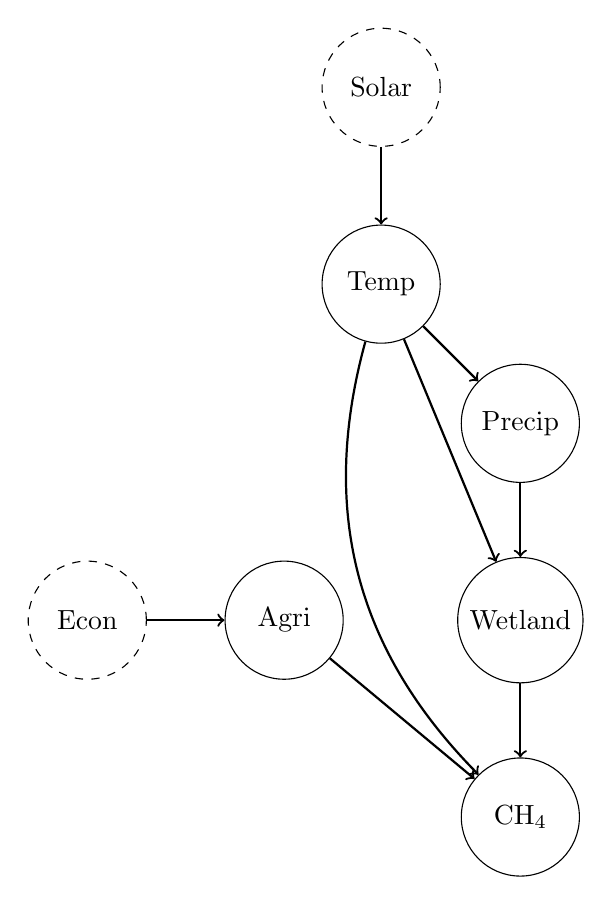
\begin{tikzpicture}[
   node distance=2.5cm,
   var/.style={circle, draw, minimum width=1.5cm},
   latent/.style={circle, draw, dashed, minimum width=1.5cm},
   arrow/.style={->, thick}
]
% Nodes
\node[var] (temp) {Temp};
\node[var] (precip) [below right of=temp] {Precip};
\node[var] (wet) [below of=precip] {Wetland};
\node[var] (agri) [left of=wet, node distance=3cm] {Agri};
\node[var] (ch4) [below of=wet] {CH$_4$};
\node[latent] (solar) [above of=temp] {Solar};
\node[latent] (econ) [left of=agri] {Econ};

% Edges
\draw[arrow] (solar) -- (temp);
\draw[arrow] (temp) -- (precip);
\draw[arrow] (temp) -- (wet);
\draw[arrow] (precip) -- (wet);
\draw[arrow] (wet) -- (ch4);
\draw[arrow] (agri) -- (ch4);
\draw[arrow] (temp) to[bend right=30] (ch4);
\draw[arrow] (econ) -- (agri);

\end{tikzpicture}
\caption{Causal graph induced by the simplified methane SCM. Solid circles represent endogenous (observed) variables, dashed circles represent exogenous factors. Edges encode direct causal relationships from structural equations.}
\label{fig:methane_dag}
\end{figure}

The graph provides visual intuition about causal relationships while maintaining mathematical precision. Path-based reasoning on the graph corresponds to algebraic manipulation of structural equations.

\subsubsection{The Modularity Principle}

A fundamental property of SCMs is modularity: each structural equation represents an autonomous mechanism that remains invariant when other mechanisms are modified. This principle, also known as autonomy or invariance, underlies the computation of interventions.

When we intervene to set $V_i = v$, we:
\begin{enumerate}
\item Replace the structural equation for $V_i$ with the constant assignment $V_i = v$
\item Keep all other structural equations unchanged
\item Compute the resulting distribution
\end{enumerate}

This "surgery" on the model corresponds to removing incoming edges to $V_i$ in the causal graph. The modularity principle asserts that intervening on one mechanism does not alter others, draining wetlands changes methane emissions but does not change how temperature affects precipitation.

\subsubsection{Computing Interventions}

The do-operator formally represents interventions in SCMs. Computing $P(Y|\text{do}(X=x))$ involves:

\begin{enumerate}
\item \textbf{Modify the SCM}: Replace the structural equation for X with X = x
\item \textbf{Compute the induced distribution}: Propagate the intervention through remaining equations
\item \textbf{Marginalize}: Sum over exogenous variables to get the interventional distribution
\end{enumerate}

For the methane example, computing the effect of wetland restoration:
\begin{align}
P(\text{CH}_4|\text{do}(\text{Wetlands}=w)) &= \sum_{t,p,a} P(\text{CH}_4|w,a,t) \\
&\quad \times P(a)P(t)P(p|t)
\end{align}

Note that precipitation's dependence on wetlands disappears under intervention, we force wetlands to value w regardless of precipitation.

\subsubsection{Counterfactual Reasoning}

SCMs enable counterfactual reasoning through their structural equations. To compute "What would methane levels have been if wetlands had been 20\% smaller?":

\begin{enumerate}
\item \textbf{Abduction}: Given observed data, infer the values of exogenous variables U
\item \textbf{Action}: Modify the model to reflect the counterfactual scenario (reduce wetlands by 20\%)
\item \textbf{Prediction}: Compute outcomes under the modified model with inferred U values
\end{enumerate}

This three-step process requires fully specified structural equations, not just the causal graph. Different functional forms can yield different counterfactual predictions even with the same graph structure.

\subsubsection{Limitations and Challenges}

While SCMs provide a powerful framework, they come with important limitations:

\textbf{Causal Sufficiency}: Standard SCMs assume no unmeasured confounders, all common causes of measured variables are included in the model. This rarely holds in environmental systems where many processes remain unobserved or unmeasurable.

\textbf{Acyclicity}: SCMs require directed acyclic graphs, yet many environmental systems exhibit feedback loops. Temperature affects methane emissions, which affect radiative forcing, which affects temperature. Extensions to cyclic models exist but complicate inference.

\textbf{Functional Form Specification}: While the causal graph may be identifiable from data, the specific functional forms of structural equations typically are not. Different functions consistent with the same graph can yield different quantitative predictions.

\textbf{Stationarity}: SCMs typically assume time-invariant relationships, yet environmental systems exhibit regime shifts, tipping points, and evolving dynamics. Climate change itself represents non-stationarity in Earth system relationships.

Despite these challenges, SCMs remain the most comprehensive framework for causal reasoning, providing the mathematical foundation for moving from correlation to causation in environmental monitoring.

\subsection{Graphical Causal Representations}

Causal relationships naturally lend themselves to graphical representation, where nodes denote variables and edges encode direct causal influences. These graphs serve multiple purposes: they make causal assumptions transparent, enable visual reasoning about complex relationships, and provide the mathematical machinery for causal inference. Different types of graphs capture different aspects of causal structure, from complete specifications to equivalence classes representing our uncertainty.

\subsubsection{Directed Acyclic Graphs (DAGs): The Foundation}

A Directed Acyclic Graph consists of nodes representing variables connected by directed edges indicating direct causal relationships. The "acyclic" constraint ensures no variable can be its own cause, even indirectly. In a DAG $G = (V, E)$, an edge $V_i \rightarrow V_j$ asserts that $V_i$ has a direct causal effect on $V_j$, an effect that persists even when controlling for all other variables in the graph.

DAGs encode independence relationships through the d-separation criterion. This graphical criterion determines which variables are conditionally independent given others, providing a complete characterization of the independence constraints implied by the causal structure. Understanding d-separation requires recognizing three basic patterns:

\textbf{Chains} ($A \rightarrow B \rightarrow C$): Information flows from A to C through B. If we condition on B (observe its value), we block this flow, making A and C independent given B. In methane systems, temperature might affect wetland extent, which affects emissions. Knowing wetland extent blocks the indirect path from temperature to emissions.

\textbf{Forks} ($A \leftarrow B \rightarrow C$): A common cause B creates correlation between A and C. Conditioning on B blocks this spurious correlation. Seasonal cycles might drive both temperature and vegetation patterns. Controlling for season removes their spurious correlation.

\textbf{Colliders} ($A \rightarrow B \leftarrow C$): Two causes converge on a common effect. Initially, A and C are independent. However, conditioning on B (or its descendants) creates correlation between A and C. If both wetlands and agriculture affect methane levels, then observing unusually high methane makes wetland and agricultural sources negatively correlated, if one is high, the other must be lower to explain the observation.

\begin{figure}[h!]
\centering
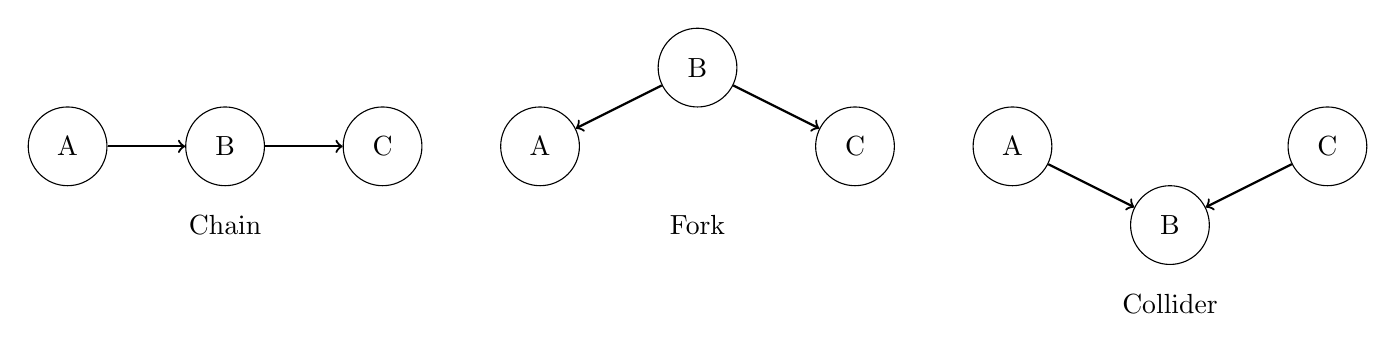
\begin{tikzpicture}[
   node distance=2cm,
   var/.style={circle, draw, minimum width=1cm},
   arrow/.style={->, thick}
]
% Chain
\node[var] (a1) at (0,0) {A};
\node
[var] (b1) at (2,0) {B};
\node[var] (c1) at (4,0) {C};
\draw[arrow] (a1) -- (b1);
\draw[arrow] (b1) -- (c1);
\node at (2,-1) {Chain};

% Fork
\node[var] (a2) at (6,0) {A};
\node[var] (b2) at (8,1) {B};
\node[var] (c2) at (10,0) {C};
\draw[arrow] (b2) -- (a2);
\draw[arrow] (b2) -- (c2);
\node at (8,-1) {Fork};

% Collider
\node[var] (a3) at (12,0) {A};
\node[var] (b3) at (14,-1) {B};
\node[var] (c3) at (16,0) {C};
\draw[arrow] (a3) -- (b3);
\draw[arrow] (c3) -- (b3);
\node at (14,-2) {Collider};

\end{tikzpicture}
\caption{Three fundamental patterns in DAGs. Chains and forks transmit correlation that conditioning blocks. Colliders block correlation until conditioning induces it.}
\label{fig:dag_patterns}
\end{figure}

The d-separation criterion formalizes these intuitions: A path between X and Y is blocked by conditioning set Z if it contains either (i) a chain or fork with the middle node in Z, or (ii) a collider with neither the collider nor its descendants in Z. Variables X and Y are d-separated by Z if all paths between them are blocked.

The power of d-separation lies in its completeness: it characterizes all conditional independence relationships implied by the causal structure. The Markov property connects graph structure to probability:
\begin{equation}
X \perp_d Y | Z \text{ in } G \implies X \perp Y | Z \text{ in } P
\end{equation}

This means d-separation in the graph implies conditional independence in any distribution compatible with the causal structure.

\subsubsection{Completed Partially Directed Acyclic Graphs (CPDAGs): Representing Equivalence}

While a true causal DAG uniquely determines independence relationships, the reverse is not true, multiple DAGs can encode the same conditional independencies. These Markov equivalent DAGs form equivalence classes, represented by CPDAGs.

A CPDAG contains:
\begin{itemize}
\item \textbf{Directed edges}: Present with the same orientation in all equivalent DAGs
\item \textbf{Undirected edges}: Oriented differently across equivalent DAGs
\end{itemize}

Two DAGs are Markov equivalent if and only if they have:
\begin{enumerate}
\item The same skeleton (underlying undirected graph)
\item The same v-structures (colliders)
\end{enumerate}

This characterization, known as the Verma-Pearl theorem, provides a complete criterion for Markov equivalence. It reveals what can and cannot be learned from observational data alone under the faithfulness assumption.

Consider three variables: Temperature (T), Wetlands (W), and Methane (M). The following DAGs are Markov equivalent:
\begin{itemize}
\item T → W → M
\item T ← W → M  
\item T ← W ← M
\end{itemize}

All share the same skeleton (T-W-M) and have no v-structures. Their CPDAG would show T, W, M with all edges undirected, indicating that observational data cannot determine causal direction without additional assumptions.

However, T → W ← M is not equivalent to the others, it contains a v-structure at W. If data shows T and M are marginally independent but become dependent when conditioning on W, this uniquely identifies the v-structure.

\begin{figure}[h!]
\centering
\begin{tikzpicture}[
   node distance=2cm,
   var/.style={circle, draw, minimum width=1cm},
   arrow/.style={->, thick},
   line/.style={-, thick}
]
% Equivalent DAGs
\node at (0,2) {Equivalent DAGs:};

% DAG 1
\node[var] (t1) at (0,0) {T};
\node[var] (w1) at (1.5,0) {W};
\node[var] (m1) at (3,0) {M};
\draw[arrow] (t1) -- (w1);
\draw[arrow] (w1) -- (m1);

% DAG 2
\node[var] (t2) at (5,0) {T};
\node[var] (w2) at (6.5,0) {W};
\node[var] (m2) at (8,0) {M};
\draw[arrow] (w2) -- (t2);
\draw[arrow] (w2) -- (m2);

% DAG 3
\node[var] (t3) at (10,0) {T};
\node[var] (w3) at (11.5,0) {W};
\node[var] (m3) at (13,0) {M};
\draw[arrow] (w3) -- (t3);
\draw[arrow] (m3) -- (w3);

% CPDAG
\node at (6,-2) {Resulting CPDAG:};
\node[var] (t4) at (5,-3.5) {T};
\node[var] (w4) at (6.5,-3.5) {W};
\node[var] (m4) at (8,-3.5) {M};
\draw[line] (t4) -- (w4);
\draw[line] (w4) -- (m4);

\end{tikzpicture}
\caption{Three Markov equivalent DAGs and their CPDAG representation. Undirected edges in the CPDAG indicate orientational uncertainty that cannot be resolved from observational data alone.}
\label{fig:cpdag_example}
\end{figure}

CPDAGs reveal a fundamental limitation: observational data, no matter how abundant, cannot fully determine causal structure. Additional assumptions (like causal ordering from temporal precedence) or interventional data are needed to orient undirected edges.

\subsubsection{Maximal Ancestral Graphs (MAGs) and Partial Ancestral Graphs (PAGs): Handling Hidden Variables}

Real-world systems invariably include unmeasured variables, subsurface processes affecting methane emissions, unobserved economic factors driving land use, or complex microbial dynamics. MAGs and PAGs extend the graphical framework to represent causal relationships in the presence of latent confounders.

A MAG uses three types of edges:
\begin{itemize}
\item \textbf{Directed} ($\rightarrow$): Direct causation
\item \textbf{Bidirected} ($\leftrightarrow$): Confounding by unmeasured common cause
\item \textbf{Undirected} (, ): Selection bias from conditioning
\end{itemize}

The bidirected edge is particularly important for environmental systems. If $X \leftrightarrow Y$, some unmeasured variable affects both. For instance, soil moisture might be unmeasured but affect both vegetation indices and methane emissions, inducing a bidirected edge between them in the MAG.

PAGs extend this further by representing equivalence classes of MAGs, analogous to how CPDAGs represent equivalence classes of DAGs. PAG edges use additional symbols:

\begin{itemize}
  \item Circle ($\circ$): Endpoint is arrow in some MAGs, tail in others
  \item Arrow ($\rightarrow$): Endpoint is arrow in all MAGs
  \item Tail ($-$): Endpoint is tail in all MAGs
\end{itemize}


Edge interpretations in PAGs:
\begin{itemize}
\item $X \rightarrow Y$: X causes Y (possibly through unmeasured mediators)
\item $X \leftrightarrow Y$: X and Y share unmeasured common cause(s)
\item $X \circ\!\rightarrow Y$: Either causal or confounded
\item $X \circ\!-\!\circ Y$: Any relationship possible
\end{itemize}

\begin{table}[h!]
\centering
\caption{Comparison of Graphical Representations}
\label{tab:graph_types}
\begin{tabular}{p{2cm}|p{3cm}|p{3cm}|p{3cm}|p{3cm}}
\hline
\textbf{Property} & \textbf{DAG} & \textbf{CPDAG} & \textbf{MAG} & \textbf{PAG} \\
\hline
Purpose & Single causal model & Equivalence class of DAGs & Single model with hidden variables & Equivalence class of MAGs \\
Edge Types & Directed only & Directed + Undirected & Directed + Bidirected + Undirected & Additional circle endpoints \\
Hidden Variables & Not represented & Not represented & Implicit in bidirected edges & Implicit with uncertainty \\
What it represents & Complete causal specification & Observational equivalence & Marginal causal structure & Marginal equivalence \\
Use Case & Known structure & Structure learning result & Known hidden confounding & Learning with hidden confounding \\
\hline
\end{tabular}
\end{table}

\subsubsection{Practical Implications for Methane Monitoring}

The choice of graphical representation depends on available knowledge and assumptions:

\textbf{Use DAGs when}:
\begin{itemize}
\item Causal relationships are well-established from domain knowledge
\item All relevant variables are measured
\item The goal is to compute specific causal effects
\item Temporal ordering provides clear causal direction
\end{itemize}

\textbf{Use CPDAGs when}:
\begin{itemize}
\item Learning causal structure from observational data
\item Some causal directions remain uncertain
\item Multiple models are equally consistent with data
\item Identifying what experiments would resolve ambiguity
\end{itemize}

\textbf{Use PAGs when}:
\begin{itemize}
\item Important variables are unmeasurable (soil microbes, economic factors)
\item Confounding is suspected but sources unknown
\item Conservative inference is needed
\item Satellite data provides incomplete system observation
\end{itemize}

For satellite-based methane monitoring, PAGs often provide the most realistic representation. We cannot measure all relevant processes, microbial populations, subsurface conditions, human decision-making, yet these latent factors certainly influence observed relationships. PAGs acknowledge this uncertainty while still enabling meaningful causal inference.

\subsection{Causal Discovery for Non-Temporal Data}

Causal discovery aims to infer causal structure from observational data, reversing the traditional statistical workflow where models are specified a priori. Rather than testing predetermined hypotheses, causal discovery algorithms systematically explore the space of possible causal structures to identify relationships consistent with observed data. This data-driven approach proves particularly valuable in complex environmental systems where complete prior knowledge is unavailable and controlled experiments are infeasible.

The fundamental challenge lies in the underdetermination problem: multiple causal structures can generate identical observational distributions. Causal discovery methods address this through different strategies, each making distinct assumptions about the data-generating process. Understanding these assumptions and their implications is crucial for appropriate method selection and interpretation.

\subsubsection{Constraint-Based Methods: Learning from Independence}

Constraint-based algorithms reconstruct causal structure by systematically testing conditional independence relationships in data. The core insight is that causal structure constrains which variables can be independent given others, these constraints, in turn, reveal the underlying causal graph.

\textbf{The PC Algorithm: Foundation of Constraint-Based Discovery}

The PC algorithm, named after its creators Peter Spirtes and Clark Glymour, exemplifies the constraint-based approach. It operates in two distinct phases:

\textbf{Phase 1: Skeleton Discovery}. Starting with a complete undirected graph, the algorithm progressively removes edges based on conditional independence tests. For each pair of variables $(X_i, X_j)$, it searches for a conditioning set $\mathbf{S}$ that renders them independent:

\begin{algorithm}[h!]
\caption{PC Algorithm: Skeleton Discovery}
\label{alg:pc-skeleton}
\begin{algorithmic}[1]
\Require Variable set $V$, initial complete undirected graph $G=(V,E)$, conditional independence oracle $\Call{IndTest}{X_i,X_j,\mathbf{S},\alpha}$, significance $\alpha$
\Ensure Undirected skeleton $G$ and separation sets $\mathrm{SepSet}[i][j]$
\State $\mathrm{SepSet}[i][j] \gets \varnothing$ for all ordered pairs $(i,j)$
\State $\ell \gets 0$
\Repeat
    \State $\mathrm{removed\_in\_level} \gets \textbf{false}$
    \ForAll{adjacent unordered pairs $\{X_i,X_j\} \subseteq V$ with $\{X_i,X_j\} \in E$}
        \State $\mathcal{A}_i \gets \Adj_G(X_i) \setminus \{X_j\}$ \Comment{Current neighbors of $X_i$ excluding $X_j$}
        \If{$|\mathcal{A}_i| \ge \ell$}
            \ForAll{$\mathbf{S} \subseteq \mathcal{A}_i \;\; \text{with } |\mathbf{S}|=\ell$}
                \If{$\Call{IndTest}{X_i,X_j,\mathbf{S},\alpha} = \textbf{independent}$}
                    \State $E \gets E \setminus \{\{X_i,X_j\}\}$ \Comment{Remove edge}
                    \State $\mathrm{SepSet}[i][j] \gets \mathbf{S}$; \quad $\mathrm{SepSet}[j][i] \gets \mathbf{S}$ \Comment{Store both directions}
                    \State $\mathrm{removed\_in\_level} \gets \textbf{true}$
                    \State \textbf{break} \Comment{Stop searching larger $\mathbf{S}$ for this pair}
                \EndIf
            \EndFor
        \EndIf
        \If{$\{X_i,X_j\} \in E \;\;\wedge\;\; |\mathcal{A}_i| < \ell$}
            \State $\mathcal{A}_j \gets \Adj_G(X_j) \setminus \{X_i\}$
            \If{$|\mathcal{A}_j| \ge \ell$}
                \ForAll{$\mathbf{S} \subseteq \mathcal{A}_j \;\; \text{with } |\mathbf{S}|=\ell$}
                    \If{$\Call{IndTest}{X_i,X_j,\mathbf{S},\alpha} = \textbf{independent}$}
                        \State $E \gets E \setminus \{\{X_i,X_j\}\}$
                        \State $\mathrm{SepSet}[i][j] \gets \mathbf{S}$; \quad $\mathrm{SepSet}[j][i] \gets \mathbf{S}$
                        \State $\mathrm{removed\_in\_level} \gets \textbf{true}$
                        \State \textbf{break}
                    \EndIf
                \EndFor
            \EndIf
        \EndIf
    \EndFor
    \State $\ell \gets \ell + 1$
\Until{$\mathrm{removed\_in\_level} = \textbf{false}$ \textbf{ or } $\max_{X \in V} |\Adj_G(X)| < \ell$}
\State \Return $G,\ \mathrm{SepSet}$
\end{algorithmic}
\end{algorithm}


The algorithm exploits efficiency by testing conditioning sets of increasing size, stopping when independence is detected. This staged approach dramatically reduces computational complexity compared to testing all possible conditioning sets.

\textbf{Phase 2: Orientation}. With the skeleton established, the algorithm orients edges to create a DAG. The fundamental rule identifies v-structures:

If the skeleton contains $X_i - X_k - X_j$ with $X_i$ and $X_j$ non-adjacent, and $X_k \notin \mathbf{S}_{ij}$, then orient as $X_i \rightarrow X_k \leftarrow X_j$.

The logic is compelling: if $X_k$ were not a collider, it would d-separate $X_i$ and $X_j$, so it should appear in their separation set. Its absence indicates a v-structure.

Meek's orientation rules complete the process, propagating orientations while maintaining acyclicity:

\begin{figure}[h!]
\centering
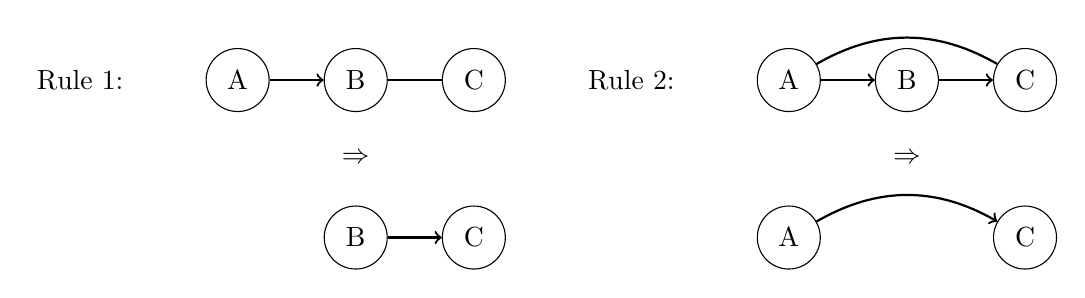
\begin{tikzpicture}[
   node distance=1.5cm,
   var/.style={circle, draw, minimum width=0.8cm},
   arrow/.style={->, thick},
   line/.style={-, thick}
]
% Meek Rule 1
\node at (0,0) {Rule 1:};
\node[var] (a1) at (2,0) {A};
\node[var] (b1) at (3.5,0) {B};
\node[var] (c1) at (5,0) {C};
\draw[arrow] (a1) -- (b1);
\draw[line] (b1) -- (c1);
\node at (3.5,-1) {$\Rightarrow$};
\node[var] (b1b) at (3.5,-2) {B};
\node[var] (c1b) at (5,-2) {C};
\draw[arrow] (b1b) -- (c1b);

% Meek Rule 2
\node at (7,0) {Rule 2:};
\node[var] (a2) at (9,0) {A};
\node[var] (b2) at (10.5,0) {B};
\node[var] (c2) at (12,0) {C};
\draw[arrow] (a2) -- (b2);
\draw[arrow] (b2) -- (c2);
\draw[line] (a2) to[bend left=30] (c2);
\node at (10.5,-1) {$\Rightarrow$};
\node[var] (a2b) at (9,-2) {A};
\node[var] (c2b) at (12,-2) {C};
\draw[arrow] (a2b) to[bend left=30] (c2b);

\end{tikzpicture}
\caption{Meek's orientation rules. Rule 1 prevents new v-structures; Rule 2 prevents cycles. Additional rules handle more complex patterns.}
\label{fig:meek_rules}
\end{figure}

\textbf{Statistical Testing Considerations}

The choice of conditional independence test critically affects performance:

\begin{itemize}
\item \textbf{Partial correlation} (Gaussian assumption): Tests whether the partial correlation $\rho_{XY|Z}$ equals zero
\item \textbf{Mutual information} (nonparametric): Tests whether $I(X;Y|Z) = 0$
\item \textbf{Kernel-based tests} (nonlinear): Use reproducing kernel Hilbert spaces to detect complex dependencies
\end{itemize}

Multiple testing presents a significant challenge. With hundreds of variables, the algorithm performs thousands of tests, inflating false discovery rates. Modern implementations use false discovery rate (FDR) control or stability selection to address this issue.

\textbf{The FCI Algorithm: Handling Latent Confounders}

The Fast Causal Inference (FCI) algorithm extends PC to scenarios with unmeasured confounders. It produces PAGs rather than DAGs, acknowledging uncertainty from hidden variables.

FCI's key innovation is conditioning on possible ancestors rather than just adjacent nodes. This broader conditioning set can d-separate variables even when confounders create spurious adjacencies in the observed graph. The algorithm adds orientation rules specific to ancestral graphs, distinguishing between direct causation and confounding.

For methane systems where microbial processes, subsurface conditions, and human decisions remain unmeasured, FCI provides more reliable inference than PC, though at increased computational cost.

\subsubsection{Score-Based Methods: Optimization Over Graph Space}

Score-based methods formulate causal discovery as an optimization problem: find the graph that best explains the observed data according to some scoring criterion. This approach transforms the combinatorial problem of graph search into a more tractable optimization framework.

\textbf{Scoring Functions: Balancing Fit and Complexity}

The Bayesian Information Criterion (BIC) exemplifies score-based approaches:
\begin{equation}
\text{BIC}(G) = \log P(\mathbf{D}|\hat{\theta}_G, G) - \frac{k_G \log n}{2}
\end{equation}

The first term measures how well graph $G$ with maximum likelihood parameters $\hat{\theta}_G$ fits data $\mathbf{D}$. The second term penalizes complexity, where $k_G$ counts free parameters and $n$ is sample size.

For Gaussian distributions with linear relationships:
\begin{equation}
\text{BIC}(G) = -\frac{n}{2} \log|\hat{\Sigma}| - \frac{k_G \log n}{2}
\end{equation}

where $\hat{\Sigma}$ is the empirical covariance matrix and $k_G = |E| + p$ for $|E|$ edges and $p$ variables.

Alternative scoring functions include:
\begin{itemize}
\item \textbf{AIC}: Uses penalty $2k_G$ (less aggressive than BIC)
\item \textbf{BGe score}: Bayesian score with Gaussian likelihood and Wishart prior
\item \textbf{BDeu score}: Bayesian Dirichlet score for discrete variables
\end{itemize}

\textbf{Greedy Equivalence Search (GES): Efficient Optimization}

Exhaustive search over all possible DAGs is computationally intractable, the number of DAGs grows super-exponentially with variables. GES navigates this space efficiently through greedy local search.

GES operates in two phases:

\textbf{Forward phase}: Starting from an empty graph, repeatedly add the edge that maximally increases the score, continuing until no improvement is possible.

\textbf{Backward phase}: Remove edges that increase the score (noting that removing edges can increase penalized scores by reducing complexity).

The algorithm's power comes from score decomposability:
\begin{equation}
\mathcal{S}(G) = \sum_{i=1}^{p} \mathcal{S}_i(X_i, \text{PA}_i^G)
\end{equation}

This allows local computation of score changes without re-evaluating the entire graph. Adding edge $X_j \rightarrow X_i$ only affects the local score for $X_i$.

GES provides theoretical guarantees: under faithfulness and correct model specification, it consistently recovers the true CPDAG as sample size increases. Recent variants like Fast GES (FGES) incorporate parallelization and caching for improved scalability.

\subsubsection{Functional Causal Models: Exploiting Asymmetry}

Functional causal model approaches leverage asymmetries in the joint distribution to identify causal direction. While correlation is symmetric, causation often introduces detectable asymmetries in how variables relate.

\textbf{Linear Non-Gaussian Acyclic Model (LiNGAM): Identifiability through Non-Gaussianity}

LiNGAM achieves what seems impossible: unique identification of the causal DAG from observational data, without equivalence classes. The key insight is that non-Gaussianity breaks the symmetry that makes linear Gaussian models unidentifiable.

The model assumes:
\begin{equation}
\mathbf{x} = \mathbf{B}\mathbf{x} + \mathbf{e}
\end{equation}

where $\mathbf{B}$ is strictly lower-triangular (encoding causal ordering) and $\mathbf{e}$ contains independent non-Gaussian noise.

Rewriting: $\mathbf{x} = (\mathbf{I} - \mathbf{B})^{-1}\mathbf{e} = \mathbf{A}\mathbf{e}$

Independent Component Analysis (ICA) can recover $\mathbf{A}$ (up to permutation and scaling) from observed $\mathbf{x}$. The permutation that makes $\mathbf{W} = \mathbf{A}^{-1}$ lower-triangular reveals the causal ordering.

The algorithm proceeds:
\begin{enumerate}
\item Apply ICA to recover mixing matrix $\mathbf{A}$
\item Find permutation making $\mathbf{W} = \mathbf{A}^{-1}$ maximally lower-triangular
\item Set $\mathbf{B} = \mathbf{I} - \mathbf{W}$ to obtain causal structure
\end{enumerate}

For methane systems, LiNGAM could uniquely identify whether temperature drives emissions or emissions affect local temperature (through radiative effects), provided relationships are approximately linear and noise is non-Gaussian, often satisfied with log-transformed environmental variables.

\textbf{Additive Noise Models (ANM): Nonlinear Identification}

ANMs extend the identifiability principle to nonlinear relationships:
\begin{equation}
Y = f(X) + N_Y, \quad N_Y \perp X
\end{equation}

The key insight: in the correct causal direction, the residual noise is independent of the input. In the wrong direction, the backward model $X = g(Y) + N_X$ will generally have $N_X$ dependent on $Y$.

The identification principle relies on the genericity argument: for most nonlinear functions $f$ and noise distributions, the independence holds only in the true causal direction. Exceptions exist (e.g., linear Gaussian case) but are measure-zero in the space of possible models.

The algorithm tests both directions:
\begin{enumerate}
\item Regress $Y$ on $X$: $\hat{f} = \arg\min_f \mathbb{E}[(Y - f(X))^2]$
\item Test independence: $N_Y = Y - \hat{f}(X)$ independent of $X$?
\item Repeat with $X$ on $Y$
\item Select direction with better independence
\end{enumerate}

Regression uses nonparametric methods (kernel regression, Gaussian processes) to avoid functional form assumptions. Independence testing employs kernel-based tests (HSIC) or information-theoretic measures.

\textbf{Post-Nonlinear Models (PNL): Additional Flexibility}

PNL models add further flexibility:
\begin{equation}
Y = g(f(X) + N_X) + N_Y
\end{equation}

This captures scenarios where measurement processes introduce additional nonlinearity. While more flexible, PNL models are harder to identify and require stronger assumptions or larger sample sizes.

\subsubsection{Practical Considerations for Method Selection}

Choosing appropriate causal discovery methods requires understanding their assumptions, strengths, and limitations:

\begin{table}[h!]
\centering
\caption{Comparison of Causal Discovery Approaches for Methane Monitoring}
\label{tab:discovery_methods}
\begin{tabular}{p{2.5cm}|p{3.5cm}|p{3.5cm}|p{3.5cm}}
\hline
\textbf{Method} & \textbf{Key Assumptions} & \textbf{Strengths} & \textbf{Limitations} \\
\hline
PC/FCI & Faithfulness, causal Markov & Nonparametric, handles latent variables (FCI) & Multiple testing, sensitive to violations \\
GES/FGES & Correct model specification & Theoretically consistent, efficient search & Parametric assumptions, local optima \\
LiNGAM & Linear, non-Gaussian, acyclic & Unique identification & Linearity restriction \\
ANM & Additive noise, generic functions & Handles nonlinearity & Pairwise only, additivity assumption \\
\hline
\end{tabular}
\end{table}

For satellite-based methane monitoring, a hybrid approach often works best:
\begin{enumerate}
\item Apply FCI for initial structure discovery, acknowledging unmeasured confounders
\item Use ANM to orient edges where nonlinear relationships are suspected
\item Validate findings with domain knowledge and temporal constraints
\item Test robustness across methods and subsamples
\end{enumerate}

The convergence of evidence across multiple methods with different assumptions strengthens confidence in discovered relationships. Discrepancies highlight where assumptions may be violated or data insufficient, guiding further investigation.

\subsection{Causal Discovery for Temporal Data}
\label{subsec:temporal_causal}

Temporal data fundamentally changes the causal discovery problem. Time's arrow provides natural constraints, causes precede effects, while introducing new challenges through autocorrelation, dynamic relationships, and varying time scales. For satellite-based methane monitoring, where observations unfold as time series of atmospheric concentrations, emissions, and environmental drivers, temporal methods become essential for understanding system dynamics.

The temporal setting offers both opportunities and complications. Unlike static data where causal direction must be inferred from distributional asymmetries, temporal precedence provides clear directional information. However, autocorrelation can create spurious relationships, different processes operate at different time scales, and feedback loops violate the acyclicity assumption central to many methods. Successfully navigating these challenges requires specialized approaches that exploit temporal structure while accounting for its complexities.

\subsubsection{Granger Causality: The Predictive Framework}

Granger causality, introduced by Nobel laureate Clive Granger in 1969, operationalizes causation through prediction: X causes Y if past values of X help predict future values of Y beyond what Y's own past provides \cite{Granger}. This predictive notion, while not equivalent to true causation, provides a practical framework for identifying directed dependencies in time series.

\textbf{Mathematical Foundation}

Consider two time series $\{X_t\}$ and $\{Y_t\}$. The bivariate vector autoregressive (VAR) model of order $p$ captures their joint dynamics:

\begin{equation}
\begin{bmatrix} Y_t \\ X_t \end{bmatrix} = \begin{bmatrix} c_Y \\ c_X \end{bmatrix} + \sum_{i=1}^{p} \begin{bmatrix} a_{11}^{(i)} & a_{12}^{(i)} \\ a_{21}^{(i)} & a_{22}^{(i)} \end{bmatrix} \begin{bmatrix} Y_{t-i} \\ X_{t-i} \end{bmatrix} + \begin{bmatrix} \varepsilon_{Y,t} \\ \varepsilon_{X,t} \end{bmatrix}
\end{equation}

where $\boldsymbol{\varepsilon}_t \sim \mathcal{N}(0, \boldsymbol{\Sigma})$ represents innovation noise.

X Granger-causes Y if the coefficients $a_{12}^{(i)}$ are jointly non-zero. Formally, we test:
\begin{align}
H_0&: a_{12}^{(1)} = a_{12}^{(2)} = ... = a_{12}^{(p)} = 0 \\
H_1&: \exists i \text{ such that } a_{12}^{(i)} \neq 0
\end{align}

This hypothesis is tested using an F-statistic comparing the restricted model (without X) to the full model:
\begin{equation}
F = \frac{(\text{RSS}_R - \text{RSS}_U)/p}{\text{RSS}_U/(T-2p-1)}
\end{equation}

where RSS denotes residual sum of squares, subscripts R and U indicate restricted and unrestricted models, and T is the time series length.

\textbf{The Granger Causality Index}

Beyond binary testing, the strength of Granger causality can be quantified:
\begin{equation}
\mathcal{F}_{X \rightarrow Y} = \ln\left(\frac{\text{var}(\varepsilon_Y^R)}{\text{var}(\varepsilon_Y^U)}\right)
\end{equation}

This index measures the logarithmic reduction in prediction error variance when including X. For methane applications, it quantifies how much knowing temperature history improves emission prediction beyond autocorrelation alone.

\textbf{Limitations and Interpretations}

Granger causality differs from true causality in important ways:

\begin{enumerate}
\item \textbf{Confounding}: Common drivers create spurious Granger causality. Seasonal cycles might make temperature Granger-cause vegetation indices without direct causal influence.

\item \textbf{Mediation}: Indirect paths register as Granger causality. Temperature might Granger-cause methane through intermediate soil moisture effects.

\item \textbf{Instantaneous effects}: Granger causality misses contemporaneous relationships occurring within the sampling interval.

\item \textbf{Nonlinearity}: Linear VAR models miss nonlinear dependencies common in environmental systems.
\end{enumerate}

Despite limitations, Granger causality remains valuable for initial exploration of temporal dependencies, particularly when combined with domain knowledge to interpret results.

\textbf{Extensions to Address Limitations}

Modern extensions address various limitations:

\textbf{Nonlinear Granger Causality} using kernel methods \cite{Marinazzo2008}:
\begin{equation}
\mathcal{F}_{X \rightarrow Y}^{\text{kernel}} = \frac{1}{2}\ln\left(\frac{\det(\mathbf{K}_{YY})}{\det(\mathbf{K}_{YY|X})}\right)
\end{equation}

where $\mathbf{K}$ represents Gram matrices in reproducing kernel Hilbert space, capturing nonlinear dependencies.

\textbf{Spectral Granger Causality} decomposes causality by frequency:
\begin{equation}
\mathcal{F}_{X \rightarrow Y}(\omega) = -\ln\left(1 - \frac{|\mathbf{H}_{YX}(\omega)|^2 \sigma_X^2}{\mathbf{S}_{YY}(\omega)}\right)
\end{equation}

This reveals whether causality operates at fast (daily weather) or slow (seasonal) time scales.

\textbf{Conditional Granger Causality} controls for confounders:
\begin{equation}
\mathcal{F}_{X \rightarrow Y|Z} = \ln\left(\frac{\text{var}(\varepsilon_Y | Z)}{\text{var}(\varepsilon_Y | X,Z)}\right)
\end{equation}

Essential when multiple drivers (temperature, precipitation, human activity) jointly influence methane.

\subsubsection{Information-Theoretic Approaches: Beyond Linear Prediction}

Information theory provides a model-free framework for detecting causal relationships in time series. Rather than assuming specific functional forms, these methods quantify directed information flow between variables, capturing both linear and nonlinear dependencies.

\textbf{Transfer Entropy: Directed Information Flow}

Transfer entropy (TE), introduced by Schreiber \cite{Schreiber2000}, quantifies the reduction in uncertainty about the next state of $Y$ when the past of $X$ is taken into account, beyond the information already contained in $Y$'s own history. Unlike Granger causality, TE does not assume linearity or Gaussianity, making it particularly suitable for nonlinear and threshold-driven processes common in atmospheric and ecological systems.

Formally, for history vectors $\mathbf{X}^{(k)}_{t-\tau}=(X_{t-\tau},...,X_{t-k\tau})$ and $\mathbf{Y}^{(l)}_{t-\tau}=(Y_{t-\tau},...,Y_{t-l\tau})$, the lag-$\tau$ transfer entropy is:
\begin{equation}
T_{X \rightarrow Y}^{(\tau)} = H(Y_t | \mathbf{Y}^{(l)}_{t-\tau}) - H(Y_t | \mathbf{Y}^{(l)}_{t-\tau},\mathbf{X}^{(k)}_{t-\tau}),
\end{equation}
where $H(\cdot)$ denotes Shannon entropy. 

Equivalently, TE can be expressed as a conditional mutual information:
\begin{equation}
T_{X \rightarrow Y}^{(\tau)} = I(Y_t; \mathbf{X}^{(k)}_{t-\tau} \mid \mathbf{Y}^{(l)}_{t-\tau}).
\end{equation}

A positive value $T_{X \rightarrow Y}^{(\tau)}>0$ indicates that including $X$'s past reduces the uncertainty of predicting $Y_t$, thus signaling a directional dependence. In methane monitoring, TE can capture, for example, how vegetation indices provide nonlinear predictive information about methane variability beyond seasonal autocorrelation.

\textbf{Estimation and Applications}

TE estimation in continuous, autocorrelated systems typically employs $k$-nearest-neighbour entropy estimators \cite{Kraskov2004} or kernel density methods. Statistical significance is assessed via surrogate time series, such as phase-randomised surrogates, which preserve autocorrelation but destroy directional coupling. These tests are critical in atmospheric contexts where strong seasonality can otherwise induce spurious TE.

Applications of TE in geosciences include quantifying nonlinear links between ENSO indices and rainfall \cite{tongal_forecasting_2021}, ecosystem-climate interactions \cite{Benocci2025}, and Arctic methane emissions under permafrost thaw \cite{Knox2024}. Its ability to detect episodic and nonlinear events, such as fire-driven methane release, makes TE a valuable complement to Granger causality.

\subsubsection{PCMCI: Scalable Causal Networks in Time Series}

While Granger causality and transfer entropy operate primarily in low-dimensional or pairwise settings, large-scale Earth observation datasets demand methods that handle many variables, strong autocorrelation, and hidden confounding. The PCMCI (Peter and Clark Momentary Conditional Independence) algorithm \cite{Runge2019} addresses these challenges by combining constraint-based causal discovery with temporal independence testing.

\textbf{Algorithmic Steps}

PCMCI proceeds in two stages:

\begin{enumerate}
\item \textbf{Condition Selection (PC$_1$)}: For each candidate link $X_{t-\tau}^i \rightarrow Y_t^j$, the algorithm selects potential parents $\hat{P}(Y_t^j)$ by iteratively testing conditional independencies:
\begin{equation}
H_0: X_{t-\tau}^i \perp Y_t^j \; | \; \mathbf{S},
\end{equation}
where $\mathbf{S}$ is an increasing set of potential parents. Edges failing independence are removed.
\item \textbf{Momentary Conditional Independence (MCI)}: Surviving candidates are tested using an augmented conditioning set that includes both $\hat{P}(Y_t^j)$ and $\hat{P}(X_{t-\tau}^i)$ (excluding $X_{t-\tau}^i$ itself), reducing spurious detection from autocorrelation.
\end{enumerate}

Significant links are oriented to respect temporal precedence, resulting in a lag-specific causal graph.

\textbf{Strengths and Relevance}

PCMCI has three crucial advantages for methane applications:

\begin{itemize}
\item It scales to high-dimensional datasets such as MODIS land cover classes, meteorological drivers, and TROPOMI methane retrievals.
\item It explicitly accounts for autocorrelation, which is strong in atmospheric time series.
\item It allows detection of both direct and indirect pathways, distinguishing, for instance, between temperature $\rightarrow$ soil moisture $\rightarrow$ methane and direct temperature $\rightarrow$ methane effects.
\end{itemize}

Extensions such as PCMCI+ resolve contemporaneous effects, while LPCMCI incorporates latent confounding, producing Partial Ancestral Graphs (PAGs).

\textbf{Applications}

Runge et al.~\cite{Runge2019_2} applied PCMCI to global climate networks, successfully disentangling drivers of ENSO dynamics. In methane studies, PCMCI has identified lagged wetland-to-\ch{CH_4} feedbacks with typical delays of 2–3 months \cite{Krich2020}, and guided causality-aware machine learning of boreal wetland emissions \cite{Knox2024}. These results underscore PCMCI’s suitability for satellite-based methane attribution.

\subsubsection{Synthesis of Temporal Causal Methods}

Each temporal method captures different aspects of causality: Granger causality excels in linear, stationary prediction; transfer entropy reveals nonlinear directional information; PCMCI scales to multivariate, autocorrelated systems. For robust inference in methane monitoring, we adopt a triangulation strategy combining these approaches, consistent with recent advances in causal machine learning \cite{Kaddour2022}. Agreement across methods increases confidence in inferred causal links, while divergence highlights sensitivity to assumptions or data limitations.


%%%%%%%%%%%%%%%%%%%%%%%%%%%%%%%%%%%%%%%%



\section{Problem Statement}
\label{sec:problem-statement}

\subsection{Scientific and Societal Context}

Methane (\ch{CH_4}) is a key climate forcer, with radiative effects and feedbacks that significantly amplify global warming. While it has a shorter atmospheric lifetime than carbon dioxide, its near-term radiative forcing is considerably stronger, and it exhibits complex temporal and spatial variability due to its diverse emission sources, including wetlands, agriculture, fossil fuels, and biomass burning. The accurate monitoring, attribution, and regulation of \ch{CH_4} emissions are essential for meeting national and international climate targets.

Recent advances in satellite-based remote sensing, particularly through missions such as TROPOMI (Sentinel-5P), GOSAT, and GHGSat, have enabled high-resolution observation of atmospheric methane over large spatial domains. However, most studies leveraging these data remain grounded in correlational or descriptive analyses. These methods are often blind to the underlying mechanisms and confounding factors that govern methane variability, reducing their explanatory power and utility for targeted mitigation.

\subsection{Analytical Gaps in Existing Approaches}

The majority of current methane monitoring methodologies, whether ground-based or satellite-derived, lack an integrated analytical framework to assess cause-effect dynamics. Studies commonly report empirical associations between methane and environmental factors (e.g., temperature, land cover, season), yet do not resolve whether those associations reflect genuine causal processes or statistical artifacts induced by autocorrelation, shared trends, or omitted variables. This is especially limiting in a system governed by multiple interacting components and feedbacks.

Moreover, the lack of multivariate causal integration results in critical knowledge gaps. For example, it remains unclear whether observed methane increases in certain regions are primarily driven by anthropogenic activity, natural wetland dynamics, or changes in atmospheric transport. The inability to distinguish these pathways hinders our capacity to prioritize intervention points or assess attribution for liability or policy planning.

\subsection{Methodological Deficiencies in Current Practice}

Despite the availability of satellite data products with high spatiotemporal resolution, such as TROPOMI \ch{XCH_4} and MODIS land-cover classification, few studies have combined these datasets into unified time series analyses capable of testing causality. Existing approaches frequently:
\begin{itemize}
    \item Treat methane variability in isolation from co-variables such as \ch{CO}, \ch{NO_2}, or meteorological drivers;
    \item Average emissions across land-cover types, thereby masking dynamic cause-effect relationships;
    \item Neglect soil and surface optical properties that influence methane retrieval accuracy;
    \item Use regression or correlation analyses without addressing autocorrelation, confounding, or latent feedback mechanisms.
\end{itemize}

Such limitations severely restrict our ability to extract policy-relevant insights, and may even produce misleading conclusions about emission sources or trends.



\subsection{Research Gap}
\label{subsec:research-gap}

\textbf{Notwithstanding} recent advances in satellite‐based methane detection, no published framework yet integrates high-resolution column-averaged methane concentrations (\ch{XCH_4}) with dynamic land cover, surface conditions, and atmospheric covariates under a causal-inference paradigm.  Most existing investigations rely on correlation analysis, spatial overlays, or empirical trend comparisons, approaches that neither identify mechanistic relationships nor control for spurious associations.

Specifically, five critical gaps persist:

\begin{enumerate}
    \item \textbf{Lack of causal integration of heterogeneous datasets.}  
    Current studies do not fuse multi-sensor products, TROPOMI \ch{XCH_4}, MODIS land cover, and ancillary gases such as \ch{CO} and \ch{NO_2}, into a unified, gridded database suitable for causal discovery.  
    The parallel NetCDF extractor (\autoref{alg:step01_extract}), land-cover attachment routine (\autoref{alg:step02_add_lc}) and histogram generator (\autoref{alg:step03_histos}) close this preprocessing gap, but the resulting data cube has not yet been linked to formal causal attribution.
    
    \item \textbf{Neglect of spatiotemporal confounding and ecosystem heterogeneity.}  
    Most analyses ignore land-cover stratification when interpreting methane variability, conflating structural drivers with contextual confounders.  
    The classification workflow (\autoref{alg:step02_add_lc}) and visualisation modules (\autoref{alg:step03_histos}, \autoref{alg:step04_heatmap}) add spatial context, yet their outputs are not embedded in a multivariate causal framework.
    
    \item \textbf{Under-utilisation of formal causal-inference techniques in environmental time series.}  
    Although the Algorithms in the \ref{chapter:appendixB} already implements Granger causality, Transfer Entropy and PCMCI, these tools have not been applied in a unified design to test directed, temporally lagged relationships between methane and its drivers across land-cover classes and seasons.
    
    \item \textbf{Limited suitability of generic causal-discovery libraries for satellite data.}  
    Packages such as \texttt{tigramite}\footnote{\texttt{tigramite} (\url{https://github.com/jakobrunge/tigramite}) is a Python package for time-series causal discovery, implementing PCMCI/PCMCI+ \cite{Runge2019}.}, 
    \texttt{DoWhy}\footnote{\texttt{DoWhy} (\url{https://github.com/py-why/dowhy}) is a Python library for causal inference based on structural causal models and potential outcomes, widely used in econometrics and social sciences \cite{angell_estimating_2021}.}, 
    and \texttt{CausalImpact}\footnote{\texttt{CausalImpact} (\url{https://google.github.io/CausalImpact/}) is an R package by Google for estimating the causal effect of interventions in time series using Bayesian structural time-series models \cite{varian_big_2014}.} 
    assume regular sampling, low dimensionality and fixed observational units.  They provide no native support for geospatial filtering, land-cover stratification, or automated lag selection.  
    The complete workflow (\autoref{alg:step01_extract}-\autoref{alg:step05_health_check}) addresses these shortcomings through tailored preprocessing, validation, and domain-aware causal methods.
    
    
    \item \textbf{Absence of validation and explanatory feedback loops.}  
    Few studies propagate causally validated findings back into retrieval refinement. For example, to explain anomalously low \ch{XCH_4} over wetlands or to adjust satellite-algorithm attribution logic.  
    The dataset-validation framework (\autoref{alg:step05_health_check}) establishes the quality-control foundation required for such feedback.

\end{enumerate}

Collectively, these deficiencies constrain the derivation of robust mechanistic explanations for methane variability across ecosystems and time.  Without causal integration of multi-source satellite data and domain-specific inference methods, attribution remains uncertain, limiting both scientific understanding and the development of spatially explicit mitigation strategies.  Addressing these limitations is therefore essential to exploit the full diagnostic potential of Earth-observation records for climate-relevant gas monitoring and evidence-based policy.


%%%%%


\section{Research Objectives}
\label{sec:research-objectives}

\subsection{Main Objective}

To identify and quantify causal relationships between atmospheric methane concentrations and key environmental drivers, including land cover types, and atmospheric co-constituents, by applying statistical causal inference techniques to multivariate, satellite-based time series.

\subsection{Specific Objectives}

\begin{enumerate}
    \item \textbf{Construct a Harmonized Dataset from Multi-Sensor Sources:} Develop a reproducible pipeline to extract, align, and integrate TROPOMI \ch{XCH_4} time series with MODIS MCD12Q1 land cover and co-constituent data (e.g., \ch{CO}, \ch{NO_2}, AOD).

    \item \textbf{Apply Causal Inference Techniques to Detect Mechanistic Drivers:} Implement a suite of causal inference tools, including Granger causality, transfer entropy, and PCMCI, adapted for spatiotemporal satellite data. Evaluate lagged, direct, and indirect causal effects between methane and environmental variables.

    \item \textbf{Characterize Land Surface Influence on Methane Dynamics:} Assess how land cover class, wetland extent, vegetation cover and co-emissions affect the temporal variability and satellite retrieval of methane. This includes evaluating potential retrieval artefacts and ecological mechanisms (e.g., methanotrophy in dry periods).
    
    \item \textbf{Enable Stratified Causal Analysis by Land Cover and Region:} Perform ecosystem-specific causal analysis by stratifying methane time series according to land cover categories (e.g., croplands, wetlands, shrublands), enabling targeted hypothesis testing such as “Do wetland extents Granger-cause methane anomalies during wet seasons?”

    \item \textbf{Establish Interpretability and Attribution for Policy Use:} Provide explainable causal graphs and quantitative metrics of influence to support environmental accountability, regulatory assessments, and emission source attribution. Distinguish between genuine drivers and correlated proxies.

    \item \textbf{Apply and Study Causality-guided Machine Learning:} 

    \item \textbf{Perform a Systematic Review of Causal Methods for Remote Sensing Time Series:} Conduct a critical assessment of causal inference methods applied in environmental science, evaluating their assumptions, applicability to satellite data, and integration potential in methane monitoring protocols.

    \item \textbf{Contribute to Scientific Standards in Methane Attribution:} Promote the integration of causal analysis in operational Earth observation by developing reproducible methodologies and tools. Align the outputs with ESA and IPCC priorities for improving methane source detection, quantification, and policy relevance.

    \item \textbf{Develop a causality-framework software for temporal series:} Promote 

\end{enumerate}

These objectives reflect the current scope and direction of an ongoing research project and may be refined as new findings, challenges, or opportunities emerge during its development.


%%%%%

\section{Proposed Solution and Innovation}
\label{subsec:proposed-solution}

This research proposes a scalable, statistically grounded framework for causal discovery in environmental satellite time series, centered on methane. It builds on a reproducible data pipeline and combines multi-source satellite observations to address the identified gaps through:

\begin{itemize}
    \item \textbf{Unified Spatiotemporal Data Assembly:} Leveraging the existing scripts, we compile a consistent, aligned time series combining TROPOMI \ch{XCH_4} with MODIS MCD12Q1 land cover, enriched with additional products such as fire radiative power, AOD and surface temperature.

    \item \textbf{Causal Inference via Time-Lagged Statistical Tests:} Using the implemented causal series framework, we apply linear (Granger causality), non-parametric (transfer entropy), and constraint-based (PCMCI) methods to detect robust, temporally structured causal relationships between methane and its drivers. These tests explicitly account for autocorrelation, confounding, and lag structures.

    \item \textbf{Stratified Causal Analysis by Land Cover Type:} The framework enables spatial stratification by ecosystem category (e.g., croplands, wetlands) using MODIS products. This allows for targeted hypotheses, such as whether rice-dominated croplands Granger-cause methane spikes during planting periods, or whether wetland extent explains seasonal cycles.

    \item \textbf{Attribution Logic and Causal Mapping:} Directed acyclic graphs (DAGs) are constructed to model plausible causal pathways from atmospheric or land-surface variables to methane variations. This enhances the explanatory power of satellite retrievals and contributes to attribution frameworks for emissions.

    \item \textbf{Policy and Environmental Accountability:} The framework's output supports interpretability and attribution needed for emission inventories, environmental impact assessments, and legal-regulatory frameworks involving methane accountability.
\end{itemize}

This proposal differs from previous studies by not only detecting “where” methane is elevated but also identifying “why” it occurs through validated causal paths, thus transitioning from descriptive geospatial analysis to mechanistic environmental understanding.

\subsection{Scientific and Policy Relevance}
\label{subsec:scientific-relevance}

The proposed causal framework addresses a key methodological gap in satellite-based methane monitoring by:
\begin{itemize}
    \item Enabling spatiotemporally explicit attribution of methane variability to specific atmospheric and land-surface drivers;
    \item Delivering open-source, reproducible tools that integrate heterogeneous satellite data into scalable causal inference pipelines;
    \item Supporting regulatory, legal, and policy efforts that depend on scientifically validated attribution of methane sources;
    \item Aligning with the strategic priorities of ESA, the Global Methane Pledge, and IPCC initiatives that promote Earth observation for targeted climate action.
    \item Providing a transferable methodology applicable to other environmental variables (e.g., aerosols, \ch{NO_2}, vegetation indices) and domains such as hydrology, biodiversity monitoring, or urban air quality assessment.

\end{itemize}

By enhancing the interpretability and diagnostic power of satellite-derived methane products, this framework strengthens the scientific foundation for region-specific mitigation planning, improves transparency in emissions accounting, and contributes to the development of early warning systems for climate-sensitive ecosystems.




\subsection{Expected Results}

\begin{itemize}
    \item Directed acyclic graphs identifying statistically significant drivers of methane variability across land cover types.
    \item Quantified causal influence scores from environmental variables (e.g., wetland fraction, \ch{CO}, \ch{NO_2}) on \ch{XCH_4}.
    \item Spatial-temporal maps of causal links at grid-cell level or aggregated by region and season.
    \item Comparative analysis of correlation and causal analyses for linear (Granger) and nonlinear (transfer entropy, PCMCI) results to evaluate consistency.
\end{itemize}

\subsection{Scientific Contributions}

\begin{itemize}
    \item A reproducible causal inference framework for environmental satellite time series.
    \item Methodological innovation in combining land cover stratification with temporal causal tests.
    \item New empirical evidence of ecosystem-specific and seasonal methane drivers across diverse biomes.
    \item Enhanced interpretability of satellite methane retrievals for emission attribution and legal frameworks.
    \item Open-access documentation, scripts, and visual tools for the scientific community.
\end{itemize}


%%%%%

\section{Scope and Limitations}

This research focuses on leveraging satellite-based observations and causal analysis to improve the monitoring of methane emissions. The scope is confined to the analysis of atmospheric methane concentrations (XCH\textsubscript{4}) retrieved from satellite sensors, primarily TROPOMI onboard Sentinel-5P, in conjunction with environmental variables such as land cover, co-emitted gases (e.g., CO, NO\textsubscript{2}), and meteorological factors. By concentrating on globally retrieved methane concentrations, the study emphasizes relative differences and causal relationships between regions, seasons, and land cover types, rather than absolute emission flux estimates.

For instance, the focus is on identifying causal links (e.g., how changes in wetland extent or drought conditions may influence observed methane levels) rather than on precisely quantifying total emissions from each source. Several limitations are acknowledged within this defined scope.

First, this approach infers causal relationships from observational data, which inherently limits causal certainty. True causality can only be asserted under specific assumptions, such as the absence of unmeasured confounders. Since controlled experiments on the atmosphere are not feasible, the analysis relies on statistical causality tests and requires careful control of potential confounding factors (e.g., temperature variability or anthropogenic activities) that could falsely suggest causal links.

Second, the use of satellite data introduces limitations in spatial resolution and coverage. While TROPOMI provides near-daily global coverage, its resolution ($\sim$7~km) is insufficient to detect small-scale emission sources (e.g., isolated leaks or small wetland patches). This is mitigated by focusing on wide world patterns without fine-scale attribution such as pinpointing emissions from a single facility since this is beyond the scope of this study.

Additionally, satellite-derived methane concentrations are subject to measurement uncertainties and systematic biases. These may arise from cloud contamination, surface reflectance effects, or differences in retrieval algorithms. As a result, conclusions are inherently bounded by the quality and limitations of the observational data. To address this, stringent quality filters are applied, and, where feasible, multiple retrieval products are compared to ensure robustness.

Another limitation arises from methodological assumptions embedded in causal inference techniques. For example, Granger causality assumes linearity and stationarity, and relies on appropriate lag selection. These conditions may not hold uniformly across the complex and nonlinear Earth system. This study addresses such concerns by employing a suite of causality methods, including both linear and nonlinear approaches, and cross-validating their outcomes to enhance interpretive reliability.

Finally, the scope of this study is restricted to identifying drivers of atmospheric methane concentrations. It does not extend to downstream effects (e.g., climate feedbacks of methane) or to upstream social, political, or economic drivers of emissions. These broader dimensions remain outside the present analysis in order to maintain a focused investigation of observational causal relationships detectable from satellite data.


%%%%%

\section{Organization of the Document}
This document is organized into six main chapters.

\textbf{Chapter 1 (Introduction)} provides background on the problem of monitoring methane emissions, the role of causal analysis, the problem statement and research gaps, the relevance of the research, and the objectives of the study. It also outlines the scope of our work and its limitations, as well as the expected outcomes.

\textbf{Chapter 2 (Literature Review)} reviews the state of the art in relevant domains: satellite-based methane monitoring techniques, \gls{causal_inference} methods in environmental science, interactions between land cover and atmospheric composition, and existing approaches to causal analysis in time series data. Identifies findings from previous studies and highlights open challenges that motivate our research.

\textbf{Chapter 3 (Methodology)}details the methodology for this PhD project's causal analysis. It integrates established principles of causal inference, remote sensing, and computational modeling, describing the staged workflow encompassing data handling, framework validation, and large-scale satellite time series analysis. The methodology is designed to uncover robust and interpretable spatiotemporal causal relationships governing methane variability, emphasizing scalability, reproducibility, and alignment with Earth observation standards.

\textbf{Chapter 4 (Preliminary Results)} presents initial results obtained from applying parts of our framework to sample datasets and simple case studies. These early findings serve to demonstrate the feasibility of the approach and inform any necessary refinements to the methodology.

\textbf{Chapter 5 (Research Plan)} delineates the plan for the remaining research, including a timeline of activities and milestones, potential risks with mitigation strategies, and a dissemination plan for sharing results with the scientific community and stakeholders.

\textbf{Chapter 6 (Conclusion)} summarizes the contributions of the work, reflects on the findings, and discusses the limitations of the study and future work, tying the research back to the broader context and objectives outlined in the introduction.

